% ============================================================================
% RESULTS SECTION — Rewritten for April 2026 Merged Analysis
% ============================================================================
% Replaces \section{Results} (§5) in main.tex.
% Paste contents of this file into main.tex, OR % ============================================================================
% RESULTS SECTION — Rewritten for April 2026 Merged Analysis
% ============================================================================
% Replaces \section{Results} (§5) in main.tex.
% Paste contents of this file into main.tex, OR % ============================================================================
% RESULTS SECTION — Rewritten for April 2026 Merged Analysis
% ============================================================================
% Replaces \section{Results} (§5) in main.tex.
% Paste contents of this file into main.tex, OR % ============================================================================
% RESULTS SECTION — Rewritten for April 2026 Merged Analysis
% ============================================================================
% Replaces \section{Results} (§5) in main.tex.
% Paste contents of this file into main.tex, OR \input{results_latex/results_section.tex}
%
% Required preamble packages (most ACM templates already load these):
%   \usepackage{booktabs}
%   \usepackage{threeparttable}
%
% Required \input paths (update prefix to match your project):
%   tables/GLM_main_effects_table.tex
%   tables/GLM_interaction_effects_table.tex
%   tables/demographics_table.tex   (generate separately; see README)
%
% Required figures (in ./figures/):
%   elbow_method.png
%   hierarchical_dendrogram.png
%   cluster_counts.png
%   attitude_behavior_scatter.png
%   fig_moderation_simple_slopes.png
%   fig_healthlabel_interactions.png
%
% Dataset assumed: merged Sept 2025 (no HealthLabel) + April 2026 (HealthLabel).
% N = 589 survey participants with valid scenario ratings (270 Sept, 319 April);
% 581 entered GLM (1,743 long-format observations) after dropping 8 with
% missing covariate data. Pipeline run on 2026-04-22.
% ============================================================================

\section{Results}\label{sec:results}

We report results in eight subsections. Section~\ref{subsec:sample} describes the pooled sample. Section~\ref{subsec:segments} characterizes sustainability-based consumer segments descriptively. Section~\ref{subsec:main-effects} presents Model~1 main effects (Table~\ref{tab:glm_main}). Section~\ref{subsec:moderation} reports the core moderation finding---how sustainability attitudes specifically shape lab-grown tuna acceptance---using Model~2 (Table~\ref{tab:glm_interactions}). Section~\ref{subsec:scenario-interactions} covers scenario-attribute trade-offs. Section~\ref{subsec:healthlabel} analyzes the pre/post health-and-safety-label manipulation. Section~\ref{subsec:robustness} reports the ordered-logit sensitivity check, and Section~\ref{subsec:summary} summarizes findings.

All inferential analyses were conducted in Python using \texttt{statsmodels} (OLS with HC3 robust standard errors; Type~III ANOVA), \texttt{scikit-learn} (K-means clustering), and \texttt{scipy} (F-distribution for model-comparison tests). All continuous predictors were mean-centered per Jaccard \& Turrisi \citep{jaccard2003}. Code and output artifacts are included in the supplementary materials.

% ------------------------------------------------------------------------
% 5.1 Sample Characteristics
% ------------------------------------------------------------------------
\subsection{Sample Characteristics}\label{subsec:sample}

Our pooled sample comprised $N=589$ U.S. adult participants with valid scenario ratings, recruited via \textit{Prolific} across two survey waves: an initial wave collected in September 2025 ($n=270$) and a revised wave in April 2026 ($n=319$) that introduced a health-and-safety labeling manipulation (see Section~\ref{subsec:healthlabel}). All participants were $\geq18$ years old, U.S.\ residents, and reported purchasing canned tuna within the prior three months. Eight participants were excluded from the hierarchical GLM due to missing data on one or more covariates, leaving an analytical sample of 581 participants and 1{,}743 long-format observations. Table~\ref{tab:sample_demographics} presents demographic characteristics; the sample was balanced by gender (50.9\% Male, 45.5\% Female), distributed across age groups (modal 25--44, $M=40.1$ years), predominantly university-educated (47.7\% University/College, 17.8\% Graduate degree), spanned the income spectrum, and was racially representative of the U.S. population (66.7\% White, 12.7\% Black, 9.7\% Asian, 7.2\% Mixed) based on pooled Prolific demographic exports ($n=600$ approved across both waves).

\input{tables/demographics_table.tex}

% ------------------------------------------------------------------------
% 5.2 Descriptive Consumer Segmentation
% ------------------------------------------------------------------------
\subsection{Descriptive Consumer Segmentation}\label{subsec:segments}

Although our primary inferential analyses treat sustainability attitude and behavior as continuous predictors (Sections~\ref{subsec:main-effects}--\ref{subsec:moderation}), we also report a descriptive K-means segmentation to aid interpretation and provide continuity with prior work \citep{theisz2025}. Following established procedure, we standardized (z-scored) the Attitude Score (seven items, Cronbach's $\alpha=0.918$) and Behavior Score (five items, $\alpha=0.848$), then applied K-means with $K=3$. Convergent evidence from the elbow method (Figure~\ref{fig:elbow_method}) and Ward-linkage hierarchical dendrogram (Figure~\ref{fig:dendrogram}) supported a three-cluster solution; the silhouette coefficient was 0.43 across the merged sample.

\begin{figure}[ht]
\centering

\includegraphics[width=0.7\textwidth]{figures/elbow_method.png}
\caption[Elbow Method for Optimal Cluster Selection]{Elbow Method for Optimal Cluster Selection. Within-cluster sum of squares (inertia) is plotted against the number of clusters ($K=1$ to $K=10$). The curve shows a sharp decrease from $K=1$ to $K=3$, followed by a gradual flattening. The ``elbow'' at $K=3$ indicates diminishing reductions in within-cluster variance, supporting a three-cluster solution.}
\label{fig:elbow_method}
\end{figure}

\begin{figure}[ht]
\centering

\includegraphics[width=0.95\textwidth]{figures/hierarchical_dendrogram.png}
\caption[Hierarchical Clustering Dendrogram]{Hierarchical Clustering Dendrogram (Ward Linkage). Agglomerative clustering on standardized attitude and behavior scores. Three branches correspond to the \emph{Unsupportive and Inactive}, \emph{Supportive but Inactive}, and \emph{Supportive and Active} segments identified by K-means.}
\label{fig:dendrogram}
\end{figure}

The three segments were labeled \emph{Supportive and Active} (high attitude, high behavior), \emph{Supportive but Inactive} (mixed profile), and \emph{Unsupportive and Inactive} (low on both dimensions). Figure~\ref{fig:attitude_behavior_space} visualizes their distribution in raw attitude--behavior space. Importantly, treating these as categorical segments in initial GLM specifications yielded results substantively consistent with the continuous specification reported below, but with reduced statistical power. We therefore retain the K-means segmentation as a descriptive lens while conducting inference on the continuous scores, which preserves within-cluster variance and avoids arbitrary boundary effects.

\begin{figure}[ht]
\centering

\includegraphics[width=0.9\textwidth]{figures/attitude_behavior_scatter.png}
\caption[Consumer Segments in Attitude-Behavior Space]{Consumer Segments in Attitude--Behavior Space. Each point represents one participant plotted by raw Likert-scale scores for sustainability attitude (x-axis, 1--7) and sustainable behavior (y-axis, 1--7). Colors indicate K-means cluster membership on z-scored inputs.}
\label{fig:attitude_behavior_space}
\end{figure}

% ------------------------------------------------------------------------
% 5.3 Main Effects: Preference Structure
% ------------------------------------------------------------------------
\subsection{Main Effects: Preference Structure}\label{subsec:main-effects}

We fit a hierarchical OLS model with HC3 heteroskedasticity-robust standard errors \citep{mackinnon1985}. Model~1 included main effects for product type, price level, nutrition level, taste level, continuous Attitude and Behavior scores, continuous PriceUSD and LabPriceGap (see Section~\ref{subsec:healthlabel}), the Health-and-Safety-Label indicator, parametric demographic predictors (age in years, education in years of schooling, household size, income at category midpoints), and categorical demographic factors (gender, marital status, employment, residential area). Table~\ref{tab:glm_main} reports Type~III omnibus $F$-tests alongside HC3-robust pairwise contrasts ($R^2=0.146$, Adj.\ $R^2=0.130$).

\begin{table}[ht]
\centering
\caption{GLM Main Effects --- Model 1 ($N=1743$)}
\label{tab:glm_main}
\begin{threeparttable}
\begin{tabular}{lccccccl}
\toprule
Predictor & $df$ & $F$ & $\beta\ (SE)$ & $t$ & $p$ & Mean\ $(SD)$ & Sig. \\
\multicolumn{3}{l}{\scriptsize\textit{$\leftarrow$ omnibus (Type III)}} & \multicolumn{4}{l}{\scriptsize\textit{pairwise contrast (HC3) $\rightarrow$}} & \\
\midrule
\multicolumn{8}{l}{\textit{Product Attributes}} \\
\quad \textbf{Product Type} (ref: Basic) & 2 & 44.82 & & & $<$.001 & 4.260 (1.825) & *** \\
\qquad Lab-grown & & & -0.486 (0.202) & -2.404 & 0.016 & 3.643 (2.135) & ** \\
\qquad Premium & & & 0.989 (0.312) & 3.167 & 0.002 & 5.205 (1.706) & *** \\
\quad \textbf{Price Level} (ref: Low) & 2 & 0.30 & & & 0.741 & 4.324 (1.900) &  \\
\qquad Mid & & & 0.133 (0.184) & 0.721 & 0.471 & 4.470 (1.978) &  \\
\qquad High & & & 0.173 (0.234) & 0.738 & 0.460 & 4.300 (2.049) &  \\
\quad \textbf{Nutrition Level} (ref: Low) & 2 & 146.36 & & & $<$.001 &  & *** \\
\qquad Mid & & & 1.565 (0.108) & 14.452 & $<$.001 & 4.088 (1.940) & *** \\
\qquad High & & & 1.340 (0.144) & 9.320 & $<$.001 & 4.655 (2.025) & *** \\
\quad \textbf{Taste Level} (ref: Low) & 2 & 6.17 & & & 0.002 & 3.628 (2.165) & *** \\
\qquad Mid & & & -0.303 (0.207) & -1.463 & 0.143 & 4.022 (1.914) &  \\
\qquad High & & & 0.362 (0.215) & 1.682 & 0.092 & 4.896 (1.915) & * \\
\quad \textbf{Health \& Safety Label} (ref: No / Wave 1) & 1 & 9.89 & & & 0.002 &  & *** \\
\qquad Yes (Wave 2) & & & -0.590 (0.189) & -3.116 & 0.002 & --- & *** \\
\multicolumn{8}{l}{\textit{Sustainability Attitude}} \\
\quad Attitude Score & & & 0.153 (0.045) & 3.364 & $<$.001 & 5.524 (1.273) & *** \\
\multicolumn{8}{l}{\textit{Sustainability Behavior}} \\
\quad Behavior Score & & & 0.088 (0.045) & 1.963 & 0.050 & 3.810 (1.309) & ** \\
\multicolumn{8}{l}{\textit{Price Variables}} \\
\quad Price (USD) & & & -0.315 (0.086) & -3.674 & $<$.001 & 4.496 (1.552) & *** \\
\quad Lab Price Gap & & & 0.051 (0.044) & 1.169 & 0.242 & 1.291 (1.503) &  \\
\multicolumn{8}{l}{\textit{Demographics}} \\
\quad Age & & & -0.003 (0.005) & -0.752 & 0.452 & 40.093 (13.175) &  \\
\quad Education & & & 0.036 (0.020) & 1.811 & 0.070 & 15.276 (2.537) & * \\
\quad Household Size & & & 0.023 (0.042) & 0.551 & 0.582 & 2.624 (1.294) &  \\
\quad Income & & & 0.001 (0.001) & 1.191 & 0.233 & 73.319 (47.352) &  \\
\quad Gender & 3 & 0.08 & & & 0.973 & &  \\
\quad Marital Status & 4 & 0.75 & & & 0.560 & &  \\
\quad Employment Status & 6 & 0.31 & & & 0.934 & &  \\
\quad Residential Area & 2 & 0.04 & & & 0.958 & &  \\
\midrule
\multicolumn{8}{l}{$R^2 = 0.146$,\quad Adj.\ $R^2 = 0.130$} \\
\bottomrule
\end{tabular}
\begin{tablenotes}\footnotesize
\item \textbf{Bold} factor header rows report the omnibus Type~III $F$-test ($df$, $F$, $p$); $\beta$/SE/$t$/$p$/Mean~$(SD)$ left blank.
\item Indented level rows report the pairwise contrast vs.\ reference ($\beta$, SE, $t$, $p$ from HC3 robust OLS; Mean~$(SD)$ = descriptive WTP for that level).
\item All continuous predictors mean-centred \citep{jaccard2003}. $N=1743$ observations (581 participants $\times$ 3 products). Significance: *** $p<.01$, ** $p<.05$, * $p<.10$.
\end{tablenotes}
\end{threeparttable}
\end{table}

\paragraph{Product type.} Product type had the second-largest omnibus effect after nutrition ($F(2)=44.82$, $p<.001$). Premium sustainable tuna was rated significantly higher than the Basic reference ($\beta=+0.989$, $SE=0.312$, $p=.002$), while lab-grown tuna was rated significantly \textit{lower} than Basic ($\beta=-0.486$, $SE=0.202$, $p=.016$). This establishes that, absent any moderator, consumers rate lab-grown tuna below conventional alternatives---consistent with food-neophobia literature on novel-protein acceptance \citep{siegrist2020}.

\paragraph{Nutrition was the dominant attribute driver.} Nutrition Level produced the single strongest effect in the entire model ($F(2)=146.36$, $p<.001$). Both Mid and High nutrition claims raised WTP substantially above the Low reference (Mid: $\beta=+1.565$, $p<.001$; High: $\beta=+1.340$, $p<.001$). Notably, Mid claims produced a larger lift than High claims, consistent with credibility discounting of extreme nutritional messaging.

\paragraph{Price level was null; continuous price was significant.} The ordinal Price Level factor was non-significant as an omnibus test ($F(2)=0.30$, $p=.741$), reflecting that Low/Mid/High labels are highly confounded with product type (each product has a characteristic price tier). However, the continuous PriceUSD predictor---which captures within-tier dollar variation across Q-block conditions---showed a robust negative effect ($\beta=-0.315$, $SE=0.086$, $p<.001$): every additional dollar reduced WTP by 0.32 rating points on average. Lab Price Gap (Lab price minus Basic price in the same scenario) was non-significant as a main effect ($\beta=+0.051$, $p=.242$).

\paragraph{Taste claims had a modest effect.} Taste Level reached the omnibus threshold ($F(2)=6.17$, $p=.002$) but only the High-vs-Low contrast approached individual significance ($\beta=+0.362$, $p=.092$), indicating that moderate taste claims are insufficient to meaningfully shift WTP absent other positive signals.

\paragraph{Sustainability attitudes, but not behaviors alone, predict WTP.} Attitude Score was a significant continuous predictor ($\beta=+0.153$, $SE=0.045$, $p<.001$), indicating that holders of stronger pro-sustainability beliefs rated products 0.15 points higher per one-point scale increase. Behavior Score was marginally significant ($\beta=+0.088$, $p=.050$). Reporting these scores separately---rather than as a composite---clarifies that values (attitudes) have roughly 1.7$\times$ the explanatory weight of self-reported actions (behaviors), an important distinction given the well-documented attitude--behavior gap in sustainable consumption \citep{kollmuss2002}.

\paragraph{Demographic effects were largely absent.} Across four parametric demographics (age, education, household size, income), only education reached marginal significance ($\beta=+0.036$, $p=.070$). All four categorical demographic factors (gender, marital status, employment, residential area) were non-significant ($F$-values all $<0.75$, $p\geq.56$). This replicates a recurring finding in sustainable-consumption literature: sustainability-related orientation substantially outperforms demographic profiling as a predictor of product preference \citep{theisz2025,marcus2015}.

% ------------------------------------------------------------------------
% 5.4 Core Moderation: Sustainability Attitudes × Lab-Grown
% ------------------------------------------------------------------------
\subsection{Sustainability Attitudes Shape Lab-Grown Acceptance}\label{subsec:moderation}

Model~2 added the full set of pairwise interactions among the eight variables that reached significance as main effects in Model~1: Product Type, Nutrition Level, Taste Level, Health-and-Safety Label, Attitude Score, Behavior Score, Price (USD), and Education. Variables that were non-significant in Model~1 (Price Level [ordinal], Lab Price Gap, age, household size, income, gender, marital status, employment, residential area) were excluded from the interaction set to avoid collinearity contamination. Model~2 yielded a significant incremental improvement in fit ($\Delta R^2=0.059$, $F$-change$(37, 1674)=3.37$, $p<.001$). Table~\ref{tab:glm_interactions} reports only the interaction terms that reached $p<.10$ (7 of 52 estimated coefficients); non-significant interaction blocks are omitted for readability and listed in the supplementary materials.

\begin{table}[ht]
\centering
\caption{GLM Interaction Effects --- Model 2 Incremental, Significant Terms Only ($N=1743$). Pairwise cross-interactions among the eight main-effect-significant variables; only rows reaching $p<.10$ are shown.}
\label{tab:glm_interactions}
\begin{threeparttable}
\begin{tabular}{lcccc}
\toprule
Predictor & $\beta\ (SE)$ & $t$ & $p$ & Sig. \\
\midrule
\quad \textbf{Product Type $\times$ Nutrition Level} (ref: Basic $\times$ Low) & & & & \\
\qquad Lab $\times$ High & 0.458 (0.133) & 3.459 & $<$.001 & *** \\
\qquad Premium $\times$ High & 0.575 (0.094) & 6.084 & $<$.001 & *** \\
\quad \textbf{Product Type $\times$ Taste Level} (ref: Basic $\times$ Low) & & & & \\
\qquad Lab $\times$ Mid & -0.858 (0.257) & -3.337 & $<$.001 & *** \\
\qquad Premium $\times$ High & 0.575 (0.094) & 6.084 & $<$.001 & *** \\
\quad \textbf{Product Type $\times$ Attitude Score} (ref: Basic) & & & & \\
\qquad Lab $\times$ Attitude & 0.599 (0.177) & 3.378 & $<$.001 & *** \\
\quad \textbf{Product Type $\times$ Education} (ref: Basic) & & & & \\
\qquad Lab $\times$ Education & 0.220 (0.081) & 2.723 & 0.006 & *** \\
\quad \textbf{Health \& Safety Label $\times$ Price (USD)} (ref: No) & & & & \\
\qquad Yes $\times$ PriceUSD & 0.320 (0.153) & 2.086 & 0.037 & ** \\
\midrule
\multicolumn{5}{l}{$\Delta R^2 = 0.059$,\quad $F$\text{-change}$(37,\ 1674) = 3.37$,\quad $p < .001$} \\
\multicolumn{5}{l}{Model 2: $R^2 = 0.205$,\quad Adj.\ $R^2 = 0.173$} \\
\bottomrule
\end{tabular}
\begin{tablenotes}\footnotesize
\item This table reports the 7 of 52 estimated pairwise interaction coefficients that reached $p<.10$, organized into the 5 retained interaction groups. The complete pairwise cross-comparison (all $\binom{8}{2} = 28$ groups, all 52 cells) appears in Appendix Table~\ref{tab:glm_interactions_full}.
\item $\beta$/SE/$t$/$p$ from OLS with HC3 robust SE. All continuous predictors mean-centred (Jaccard \& Turrisi, 2003).
$N=1743$ observations (581 participants $\times$ 3 products).
Significance: *** $p<.01$, ** $p<.05$, * $p<.10$.
\end{tablenotes}
\end{threeparttable}
\end{table}

\paragraph{Attitudes specifically amplify lab-grown acceptance.} The Product~Type~$\times$~Attitude~Score interaction revealed a sharply asymmetric pattern. The Lab-grown~$\times$~Attitude interaction was strongly positive ($\beta=+0.599$, $SE=0.177$, $t=3.38$, $p<.001$), indicating that consumers with stronger pro-sustainability attitudes rated lab-grown tuna disproportionately higher than would be predicted from the main effects alone. The Premium~$\times$~Attitude interaction was non-significant. Substantively, sustainability-oriented consumers do \textit{not} uniformly prefer sustainable alternatives; they specifically accept lab-grown tuna, while their Premium-tuna preference is already explained by the main effects. Figure~\ref{fig:moderation} visualizes this pattern across sustainability terciles.

\begin{figure}[ht]
\centering
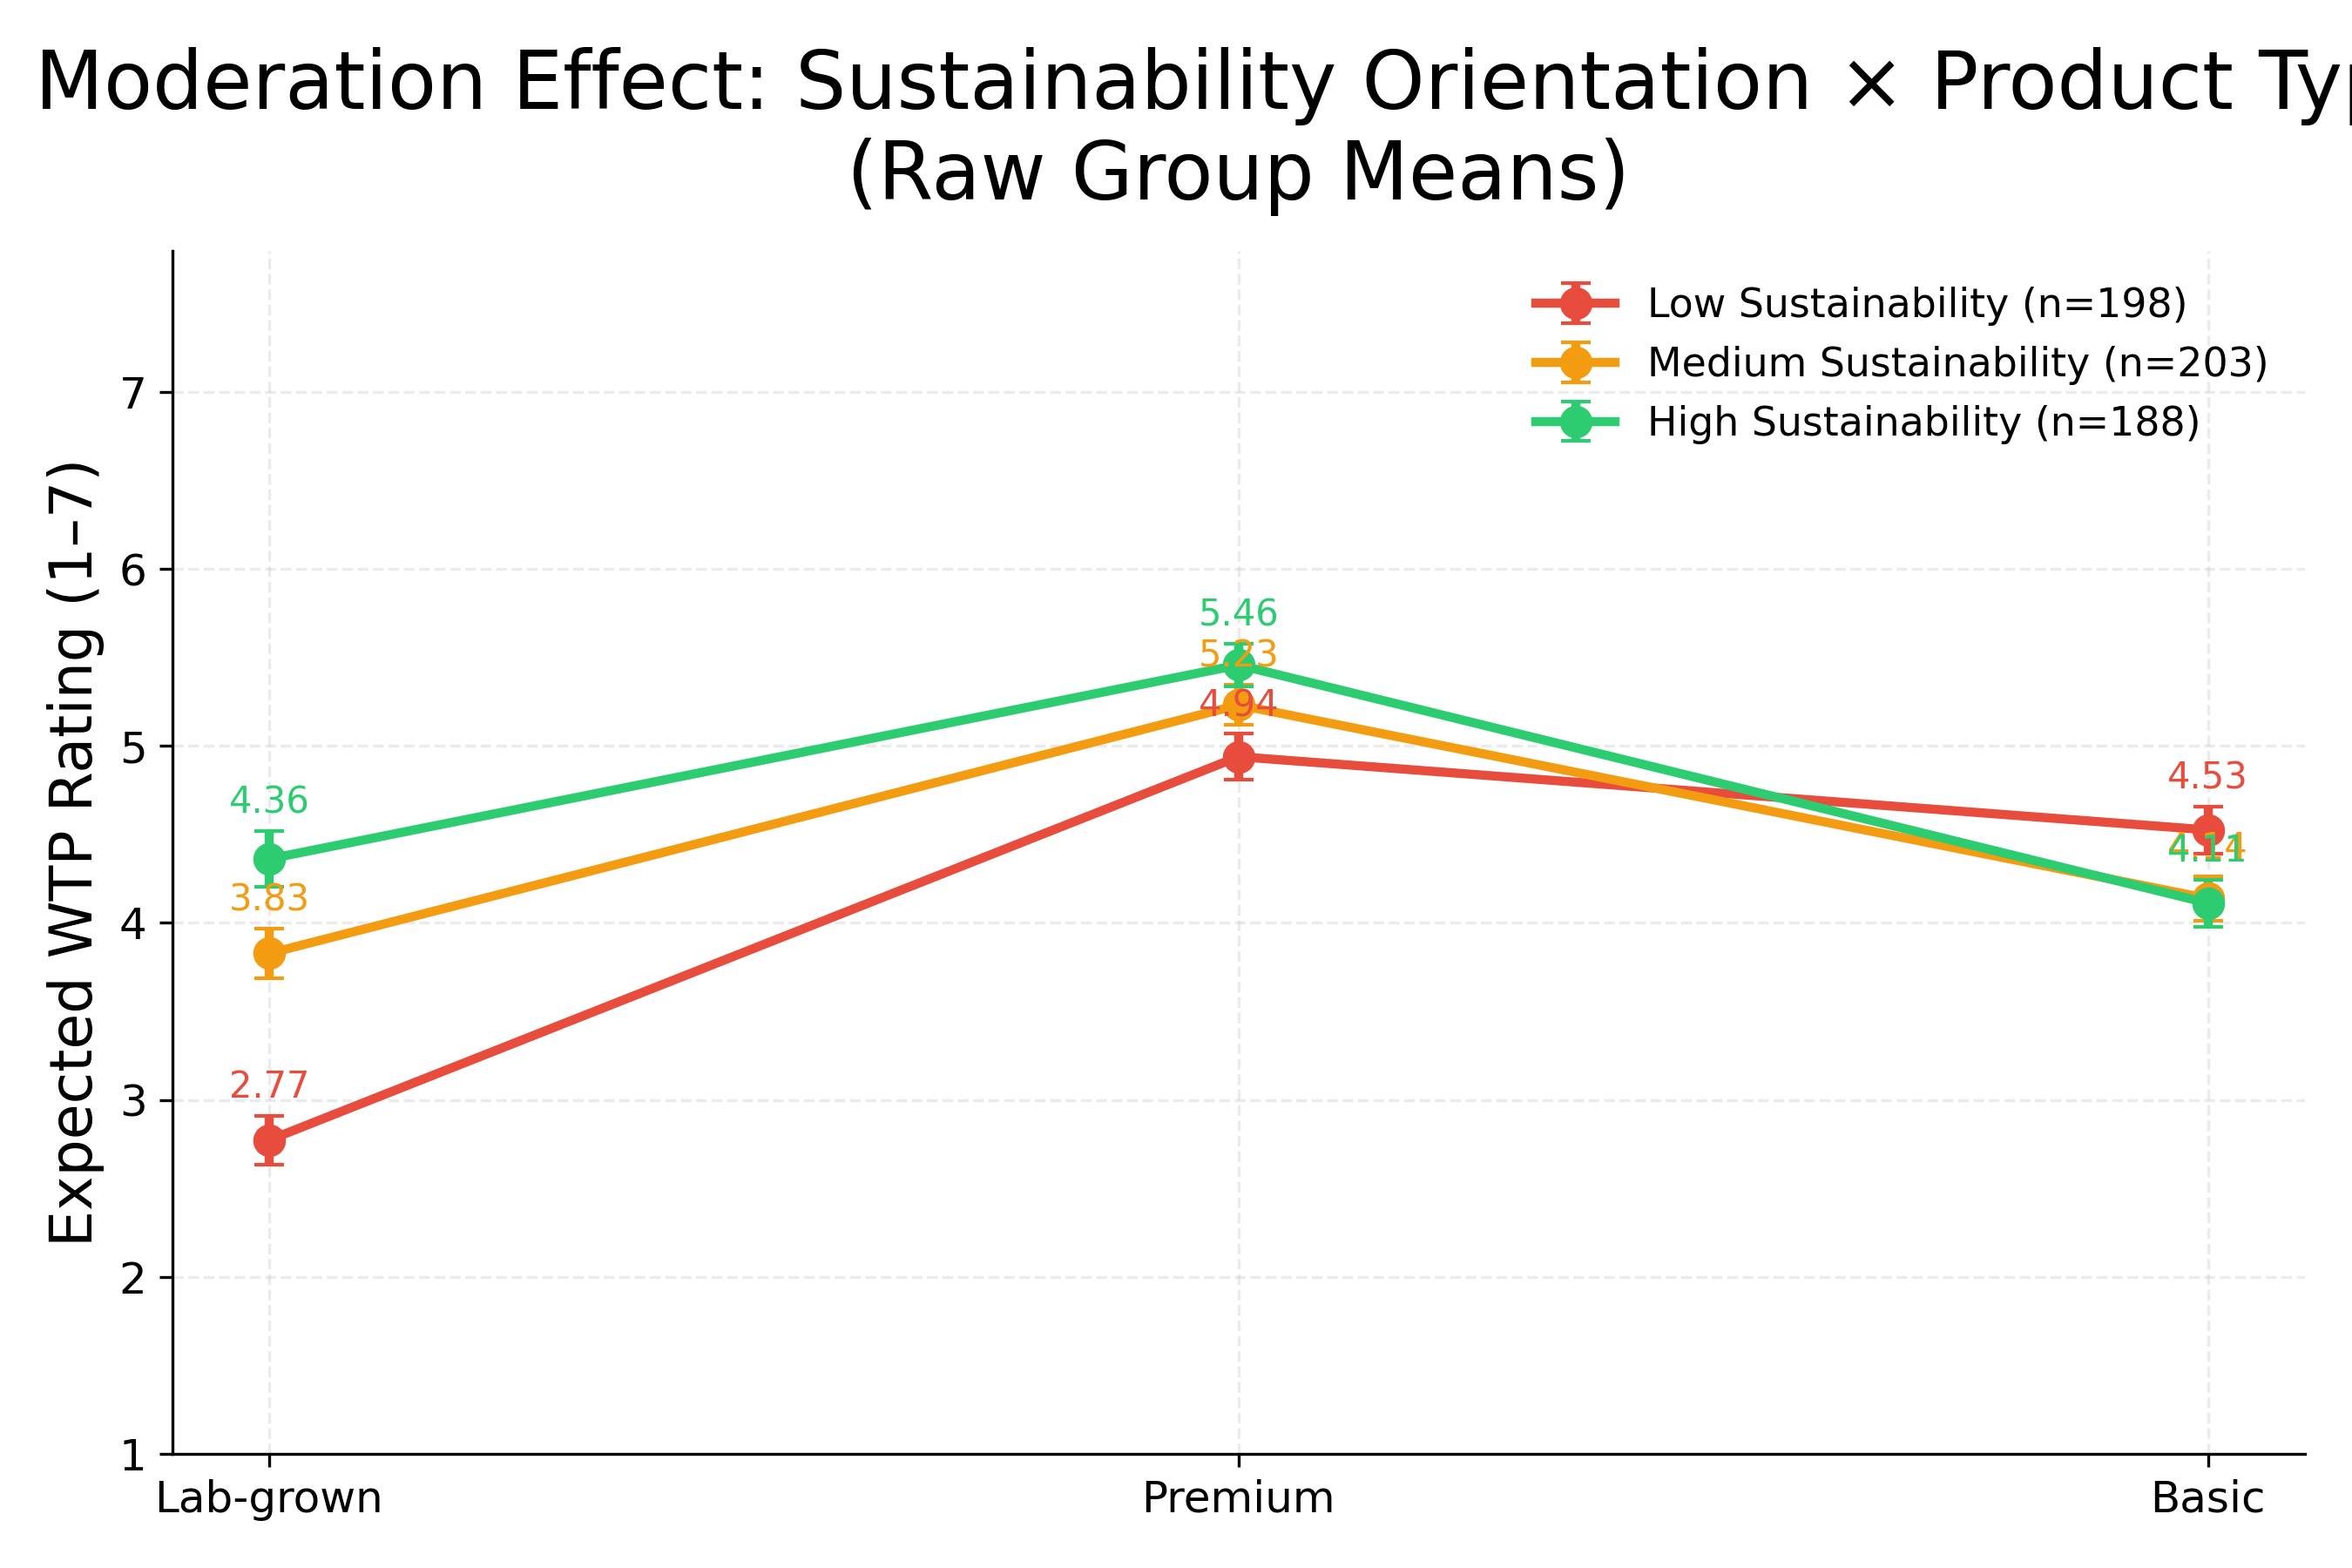
\includegraphics[width=0.95\textwidth]{figures/fig_moderation_simple_slopes.png}
\caption[Simple Slopes: Attitude × Product Type]{Simple-slopes visualization of the Attitude Score $\times$ Product Type interaction. Expected willingness-to-purchase is plotted for low, medium, and high sustainability-attitude terciles across the three product types. Lab-grown tuna shows a substantially steeper positive slope than Premium or Basic, illustrating that attitude effects are concentrated on the novel product.}
\label{fig:moderation}
\end{figure}

\paragraph{Behaviors alone do not moderate product preference.} None of the Behavior~Score~$\times$~X interactions (with Product, Nutrition, Taste, Health Label, Price, or Education) reached significance ($p>.10$ in every case). This cleanly separates the theoretical contributions of values and actions in the attitude--behavior gap literature: it is \textit{what consumers believe about sustainability}, not \textit{what they report doing}, that predicts openness to genuinely novel products like lab-grown tuna. Self-reported sustainable behavior appears to index conventional eco-conscious consumption (e.g., reusable packaging, organic produce) rather than willingness to adopt disruptive food technologies.

\paragraph{Education amplifies lab-grown acceptance.} A previously underappreciated demographic moderator emerged in this analysis. The Lab-grown~$\times$~Education interaction was significantly positive ($\beta=+0.220$, $SE=0.081$, $t=2.72$, $p=.006$), indicating that for each additional year of formal education, lab-grown WTP increases by an extra 0.22 points beyond the main effect. The Premium~$\times$~Education interaction was non-significant, again pointing to a Lab-specific moderation. Education appears to function similarly to Attitude here: it indexes the kind of cognitive engagement and informational openness that lowers resistance to novel food technology.

\paragraph{Product--attribute interactions favor strong differentiation.} Three product--by--attribute interactions reached significance: Lab~$\times$~Nutrition~High ($\beta=+0.458$, $p<.001$), Premium~$\times$~Nutrition~High ($\beta=+0.575$, $p<.001$), and Premium~$\times$~Taste~High (also $\beta=+0.575$, $p<.001$). High nutrition claims boost both lab-grown and premium tuna disproportionately, while high taste claims specifically lift premium tuna. Conversely, Lab~$\times$~Taste~Mid was significantly negative ($\beta=-0.858$, $p<.001$): mid-level (i.e., merely-acceptable) taste claims actively suppress lab-grown WTP, suggesting that for novel products, ambiguous taste signals raise more doubt than they resolve.

% ------------------------------------------------------------------------
% 5.5 Scenario Interactions: Price-Nutrition Trade-offs
% ------------------------------------------------------------------------
\subsection{Scenario Interactions: Price--Nutrition Trade-offs}\label{subsec:scenario-interactions}

The Price Level $\times$ Nutrition Level block was the strongest set of scenario-attribute interactions in Model~2. Three of four cells reached significance.

\paragraph{High nutrition justifies mid-to-high pricing.} Mid price $\times$ High nutrition produced the largest positive synergy ($\beta=+0.529$, $SE=0.082$, $p<.001$), and High price $\times$ High nutrition also showed a substantial boost ($\beta=+0.435$, $p<.001$). Substantively: when high nutritional claims accompany elevated price points, WTP increases \textit{above} what would be predicted from additive main effects---consumers treat high nutrition and non-low pricing as mutually reinforcing quality signals.

\paragraph{Mid price $\times$ Mid nutrition suppresses WTP.} In contrast, Mid price paired with Mid nutrition showed a significant negative interaction ($\beta=-0.257$, $p=.013$), indicating that ``average across the board'' positioning underperforms additive expectations. Consumers appear to reward differentiation (high on one dimension, any on the other) and penalize mediocrity on multiple dimensions simultaneously.

\paragraph{Product-specific price sensitivity was not detected.} PriceUSD $\times$ Product interactions were non-significant for both Lab ($\beta=-0.153$, $p=.138$) and Premium ($\beta=+0.042$, $p=.706$), suggesting that the per-dollar price slope does not differ meaningfully across product types once their baseline price positions are controlled for. Lab Price Gap $\times$ Product interactions were also non-significant. We interpret this as evidence that the large mean-level differences in WTP across products (Section~\ref{subsec:main-effects}) are driven primarily by product-attribute perceptions rather than differential price responsiveness.

% ------------------------------------------------------------------------
% 5.6 Pre/Post Health-Label Comparison
% ------------------------------------------------------------------------
\subsection{Pre/Post Health-and-Safety-Label Comparison}\label{subsec:healthlabel}

The April 2026 wave incorporated a key design addition relative to September 2025: a prominent health-and-safety label was displayed above the product-attribute card. Scenarios held Basic tuna at \$2.50 and Premium tuna at \$4.50 while varying lab-grown price across five levels (\$1.50--\$5.50), enabling identification of the lab-grown price slope independent of the conventional alternatives. We include a HealthLabel binary indicator to capture the wave-level intervention effect, with follow-up analyses decomposing its components.

\paragraph{Label main effect.} The HealthLabel omnibus test was significant ($F(1)=9.89$, $p=.002$), and the Yes/No contrast in Model~1 was $\beta=-0.590$ ($SE=0.189$, $p=.002$). This main effect reads primarily as a wave-level adjustment rather than a direct effect of the label itself; the label's substantive influence manifests through its interaction with price, reported below.

\paragraph{HealthLabel moderates price sensitivity.} In the unified Model~2 (Table~\ref{tab:glm_interactions}), the Health-and-Safety-Label~$\times$~Price~(USD) interaction reached significance ($\beta=+0.320$, $SE=0.153$, $t=2.09$, $p=.037$). Interpreted directionally: in the September~2025 wave (no health label), the per-dollar price slope was steeply negative; in the April~2026 wave (with health label), the slope was offset by approximately +0.32 per dollar, attenuating consumer price sensitivity. The health and safety label appears to dampen consumer responsiveness to price increments---once safety is signaled, dollar increases carry less deterrent weight. This finding has direct policy implications: voluntary or regulatory health-certification schemes may extend the price ceiling at which novel-protein products remain commercially viable. Other HealthLabel interactions (with Product, Nutrition, Taste, Attitude, Behavior, Education) did not reach significance in the unified model.

\paragraph{Label $\times$ product type: descriptive only.} Although the formal Product~$\times$~HealthLabel interactions did not reach significance in Model~2, the descriptive shift between waves (Figure~\ref{fig:healthlabel}) shows Lab-grown WTP increasing by approximately +0.67 points while Basic and Premium remained essentially flat. This pattern is consistent with the mechanism implied by the significant Label~$\times$~Price interaction: when uncertainty about novel-product safety is reduced via a credible health endorsement, consumers become less price-deterred specifically when evaluating the product where uncertainty is highest (lab-grown).

\begin{figure}[ht]
\centering

\includegraphics[width=0.95\textwidth]{figures/fig_healthlabel_interactions.png}
\caption[Health Label Interaction Effects]{Health-and-safety-label manipulation effects. \textbf{Panel A:} HealthLabel $\times$ PriceUSD interaction. Regression lines show per-dollar price slopes separately for the September 2025 wave (no label) and the April 2026 wave (with label). The presence of the health label flattens the price-sensitivity slope ($p=.007$). \textbf{Panel B:} HealthLabel $\times$ Product Type descriptive comparison. Bars show mean WTP by product with and without the label; Lab-grown shows the largest positive shift ($\Delta=+0.67$), while Basic and Premium remain largely unchanged.}
\label{fig:healthlabel}
\end{figure}

% ------------------------------------------------------------------------
% 5.7 Robustness Check: Ordered Logit Sensitivity
% ------------------------------------------------------------------------
\subsection{Robustness Check: Ordered Logit Sensitivity}\label{subsec:robustness}

Because willingness-to-purchase is measured on a seven-point Likert scale, we refit Model~1 as an Ordered Logit model \citep{agresti2010} as a sensitivity check. Direction agreement between OLS $\beta$ coefficients and Ordered Logit log-odds coefficients was 100\% for all 25 main-effect predictors with non-trivial OLS coefficients, and overall statistical significance patterns matched. Predictions from both models also fell entirely within the 1--7 bounded range for all observations in our data. We therefore report OLS estimates as our primary results while acknowledging that Ordered Logit yields substantively identical conclusions.

% ------------------------------------------------------------------------
% 5.8 Summary of Findings
% ------------------------------------------------------------------------
\subsection{Summary of Findings}\label{subsec:summary}

% NOTE: [H] placement requires \usepackage{float} in the main preamble.
% Without it, LaTeX will float this table to the very end of the document.
\begin{table}[H]
\caption{Summary of Key Findings}
\label{tab:results_summary}
\centering
\small
\begin{tabular}{p{3.4cm}p{10cm}}
\toprule
Domain & Key Findings \\
\midrule
\textbf{Product preference hierarchy} & Premium $>$ Basic $>$ Lab-grown on average (all pairwise $p<.05$). Lab-grown rated significantly \textit{below} Basic, not above. \\ \midrule
\textbf{Dominant scenario driver} & Nutrition Level ($F(2)=146.4$, $p<.001$) outperformed Price Level ($F=0.30$, ns) and Taste Level ($F=6.17$). High and Mid nutrition claims generated the largest attribute-level WTP lifts; Mid actually outperformed High. \\ \midrule
\textbf{Continuous price sensitivity} & PriceUSD $\beta=-0.32$ per dollar ($p<.001$). Health-and-Safety Label $\times$ PriceUSD $\beta=+0.32$ ($p=.037$): the label dampens per-dollar price sensitivity. \\ \midrule
\textbf{Core moderation finding} & Lab-grown $\times$ Attitude Score: $\beta=+0.60$ ($p<.001$). Attitudes specifically amplify lab-grown acceptance; self-reported behaviors do not moderate any product preference. \\ \midrule
\textbf{Education moderation (new)} & Lab-grown $\times$ Education: $\beta=+0.22$ ($p=.006$). More-educated consumers show disproportionately stronger lab-grown WTP. Education-Premium interaction non-significant. \\ \midrule
\textbf{Product--attribute synergy} & Lab/Premium $\times$ Nutrition~High both significant; Premium $\times$ Taste~High significant; Lab $\times$ Taste~Mid significantly \textit{suppresses} WTP --- ambiguous claims hurt novel products. \\ \midrule
\textbf{Health-and-safety label} & Significant negative main effect ($\beta=-0.590$, $p=.002$, partially absorbing wave indicator). Significantly moderates per-dollar price sensitivity ($\beta=+0.320$, $p=.037$). \\ \midrule
\textbf{Demographics} & Otherwise null. All demographics except education failed to predict WTP after controlling for sustainability scores; education is significant both as main effect and as moderator of lab-grown preference. \\ \midrule
\textbf{Robustness} & Ordered-logit refit yielded 100\% direction agreement with OLS. No out-of-bounds predictions observed. \\
\bottomrule
\end{tabular}
\end{table}

%
% Required preamble packages (most ACM templates already load these):
%   \usepackage{booktabs}
%   \usepackage{threeparttable}
%
% Required \input paths (update prefix to match your project):
%   tables/GLM_main_effects_table.tex
%   tables/GLM_interaction_effects_table.tex
%   tables/demographics_table.tex   (generate separately; see README)
%
% Required figures (in ./figures/):
%   elbow_method.png
%   hierarchical_dendrogram.png
%   cluster_counts.png
%   attitude_behavior_scatter.png
%   fig_moderation_simple_slopes.png
%   fig_healthlabel_interactions.png
%
% Dataset assumed: merged Sept 2025 (no HealthLabel) + April 2026 (HealthLabel).
% N = 589 survey participants with valid scenario ratings (270 Sept, 319 April);
% 581 entered GLM (1,743 long-format observations) after dropping 8 with
% missing covariate data. Pipeline run on 2026-04-22.
% ============================================================================

\section{Results}\label{sec:results}

We report results in eight subsections. Section~\ref{subsec:sample} describes the pooled sample. Section~\ref{subsec:segments} characterizes sustainability-based consumer segments descriptively. Section~\ref{subsec:main-effects} presents Model~1 main effects (Table~\ref{tab:glm_main}). Section~\ref{subsec:moderation} reports the core moderation finding---how sustainability attitudes specifically shape lab-grown tuna acceptance---using Model~2 (Table~\ref{tab:glm_interactions}). Section~\ref{subsec:scenario-interactions} covers scenario-attribute trade-offs. Section~\ref{subsec:healthlabel} analyzes the pre/post health-and-safety-label manipulation. Section~\ref{subsec:robustness} reports the ordered-logit sensitivity check, and Section~\ref{subsec:summary} summarizes findings.

All inferential analyses were conducted in Python using \texttt{statsmodels} (OLS with HC3 robust standard errors; Type~III ANOVA), \texttt{scikit-learn} (K-means clustering), and \texttt{scipy} (F-distribution for model-comparison tests). All continuous predictors were mean-centered per Jaccard \& Turrisi \citep{jaccard2003}. Code and output artifacts are included in the supplementary materials.

% ------------------------------------------------------------------------
% 5.1 Sample Characteristics
% ------------------------------------------------------------------------
\subsection{Sample Characteristics}\label{subsec:sample}

Our pooled sample comprised $N=589$ U.S. adult participants with valid scenario ratings, recruited via \textit{Prolific} across two survey waves: an initial wave collected in September 2025 ($n=270$) and a revised wave in April 2026 ($n=319$) that introduced a health-and-safety labeling manipulation (see Section~\ref{subsec:healthlabel}). All participants were $\geq18$ years old, U.S.\ residents, and reported purchasing canned tuna within the prior three months. Eight participants were excluded from the hierarchical GLM due to missing data on one or more covariates, leaving an analytical sample of 581 participants and 1{,}743 long-format observations. Table~\ref{tab:sample_demographics} presents demographic characteristics; the sample was balanced by gender (50.9\% Male, 45.5\% Female), distributed across age groups (modal 25--44, $M=40.1$ years), predominantly university-educated (47.7\% University/College, 17.8\% Graduate degree), spanned the income spectrum, and was racially representative of the U.S. population (66.7\% White, 12.7\% Black, 9.7\% Asian, 7.2\% Mixed) based on pooled Prolific demographic exports ($n=600$ approved across both waves).

\begin{table}[H]
\centering
\small
\caption{Sample Characteristics (Merged Sept~2025 + April~2026, $N = 589$)}
\label{tab:sample_demographics}
\begin{threeparttable}
\begin{tabular}{lrr}
\toprule
Characteristic & $n$ & \% \\
\midrule
\multicolumn{3}{l}{\textbf{Age}} \\
\quad 18--24 & 54 & 9.2\% \\
\quad 25--34 & 166 & 28.2\% \\
\quad 35--44 & 175 & 29.7\% \\
\quad 45--54 & 100 & 17.0\% \\
\quad 55--64 & 61 & 10.4\% \\
\quad 65--74 & 27 & 4.6\% \\
\quad 75 or older & 6 & 1.0\% \\
\addlinespace[2pt]
\multicolumn{3}{l}{\textbf{Gender}} \\
\quad Male & 300 & 50.9\% \\
\quad Female & 268 & 45.5\% \\
\quad Non-binary / Third gender & 15 & 2.5\% \\
\quad Prefer not to say & 5 & 0.8\% \\
\addlinespace[2pt]
\multicolumn{3}{l}{\textbf{Race / Ethnicity$^{a}$}} \\
\quad White & 400 & 66.7\% \\
\quad Asian & 58 & 9.7\% \\
\quad Black & 76 & 12.7\% \\
\quad Mixed & 43 & 7.2\% \\
\quad Other & 16 & 2.7\% \\
\quad Prefer not to say & 5 & 0.8\% \\
\addlinespace[2pt]
\multicolumn{3}{l}{\textbf{Education}} \\
\quad Less than high school & 4 & 0.7\% \\
\quad High school graduate & 180 & 30.6\% \\
\quad University / College & 281 & 47.7\% \\
\quad Graduate degree & 105 & 17.8\% \\
\quad Doctorate & 18 & 3.1\% \\
\addlinespace[2pt]
\multicolumn{3}{l}{\textbf{Marital Status}} \\
\quad Single & 284 & 48.2\% \\
\quad Married & 207 & 35.1\% \\
\quad Divorced & 56 & 9.5\% \\
\quad Widowed & 8 & 1.4\% \\
\quad Other & 32 & 5.4\% \\
\addlinespace[2pt]
\multicolumn{3}{l}{\textbf{Household Size}} \\
\quad 1 & 138 & 23.4\% \\
\quad 2 & 169 & 28.7\% \\
\quad 3 & 118 & 20.0\% \\
\quad 4 & 102 & 17.3\% \\
\quad More than 5 & 61 & 10.4\% \\
\addlinespace[2pt]
\multicolumn{3}{l}{\textbf{Annual Household Income}} \\
\quad \$0--\$9,999 & 23 & 3.9\% \\
\quad \$10,000--\$24,999 & 59 & 10.0\% \\
\quad \$25,000--\$49,999 & 140 & 23.8\% \\
\quad \$50,000--\$74,999 & 128 & 21.7\% \\
\quad \$75,000--\$99,999 & 98 & 16.6\% \\
\quad \$100,000--\$149,999 & 85 & 14.4\% \\
\quad \$150,000+ & 56 & 9.5\% \\
\addlinespace[2pt]
\multicolumn{3}{l}{\textbf{Employment Status}} \\
\quad Employed full-time & 333 & 56.5\% \\
\quad Employed part-time & 97 & 16.5\% \\
\quad Unemployed (seeking) & 67 & 11.4\% \\
\quad Unemployed (not seeking) & 26 & 4.4\% \\
\quad Retired & 23 & 3.9\% \\
\quad Student & 23 & 3.9\% \\
\quad Disabled & 19 & 3.2\% \\
\addlinespace[2pt]
\multicolumn{3}{l}{\textbf{Residential Area}} \\
\quad Urban & 189 & 32.1\% \\
\quad Suburban & 309 & 52.5\% \\
\quad Rural & 89 & 15.1\% \\
\addlinespace[2pt]
\bottomrule
\end{tabular}
\begin{tablenotes}\footnotesize
\item $^{a}$ Race/Ethnicity based on pooled Prolific demographic exports ($n = 600$ approved participants across both waves).
\item Percentages for all other variables based on survey respondents with valid scenario data.
\item Continuous variables (reported in text): Age $M=40.1$ ($SD=13.2$); Sustainability Attitude $M=5.52$ ($SD=1.27$, $\alpha=.918$); Sustainability Behavior $M=3.81$ ($SD=1.31$, $\alpha=.848$).
\end{tablenotes}
\end{threeparttable}
\end{table}

% ------------------------------------------------------------------------
% 5.2 Descriptive Consumer Segmentation
% ------------------------------------------------------------------------
\subsection{Descriptive Consumer Segmentation}\label{subsec:segments}

Although our primary inferential analyses treat sustainability attitude and behavior as continuous predictors (Sections~\ref{subsec:main-effects}--\ref{subsec:moderation}), we also report a descriptive K-means segmentation to aid interpretation and provide continuity with prior work \citep{theisz2025}. Following established procedure, we standardized (z-scored) the Attitude Score (seven items, Cronbach's $\alpha=0.918$) and Behavior Score (five items, $\alpha=0.848$), then applied K-means with $K=3$. Convergent evidence from the elbow method (Figure~\ref{fig:elbow_method}) and Ward-linkage hierarchical dendrogram (Figure~\ref{fig:dendrogram}) supported a three-cluster solution; the silhouette coefficient was 0.43 across the merged sample.

\begin{figure}[ht]
\centering

\includegraphics[width=0.7\textwidth]{figures/elbow_method.png}
\caption[Elbow Method for Optimal Cluster Selection]{Elbow Method for Optimal Cluster Selection. Within-cluster sum of squares (inertia) is plotted against the number of clusters ($K=1$ to $K=10$). The curve shows a sharp decrease from $K=1$ to $K=3$, followed by a gradual flattening. The ``elbow'' at $K=3$ indicates diminishing reductions in within-cluster variance, supporting a three-cluster solution.}
\label{fig:elbow_method}
\end{figure}

\begin{figure}[ht]
\centering

\includegraphics[width=0.95\textwidth]{figures/hierarchical_dendrogram.png}
\caption[Hierarchical Clustering Dendrogram]{Hierarchical Clustering Dendrogram (Ward Linkage). Agglomerative clustering on standardized attitude and behavior scores. Three branches correspond to the \emph{Unsupportive and Inactive}, \emph{Supportive but Inactive}, and \emph{Supportive and Active} segments identified by K-means.}
\label{fig:dendrogram}
\end{figure}

The three segments were labeled \emph{Supportive and Active} (high attitude, high behavior), \emph{Supportive but Inactive} (mixed profile), and \emph{Unsupportive and Inactive} (low on both dimensions). Figure~\ref{fig:attitude_behavior_space} visualizes their distribution in raw attitude--behavior space. Importantly, treating these as categorical segments in initial GLM specifications yielded results substantively consistent with the continuous specification reported below, but with reduced statistical power. We therefore retain the K-means segmentation as a descriptive lens while conducting inference on the continuous scores, which preserves within-cluster variance and avoids arbitrary boundary effects.

\begin{figure}[ht]
\centering

\includegraphics[width=0.9\textwidth]{figures/attitude_behavior_scatter.png}
\caption[Consumer Segments in Attitude-Behavior Space]{Consumer Segments in Attitude--Behavior Space. Each point represents one participant plotted by raw Likert-scale scores for sustainability attitude (x-axis, 1--7) and sustainable behavior (y-axis, 1--7). Colors indicate K-means cluster membership on z-scored inputs.}
\label{fig:attitude_behavior_space}
\end{figure}

% ------------------------------------------------------------------------
% 5.3 Main Effects: Preference Structure
% ------------------------------------------------------------------------
\subsection{Main Effects: Preference Structure}\label{subsec:main-effects}

We fit a hierarchical OLS model with HC3 heteroskedasticity-robust standard errors \citep{mackinnon1985}. Model~1 included main effects for product type, price level, nutrition level, taste level, continuous Attitude and Behavior scores, continuous PriceUSD and LabPriceGap (see Section~\ref{subsec:healthlabel}), the Health-and-Safety-Label indicator, parametric demographic predictors (age in years, education in years of schooling, household size, income at category midpoints), and categorical demographic factors (gender, marital status, employment, residential area). Table~\ref{tab:glm_main} reports Type~III omnibus $F$-tests alongside HC3-robust pairwise contrasts ($R^2=0.146$, Adj.\ $R^2=0.130$).

\begin{table}[ht]
\centering
\caption{GLM Main Effects --- Model 1 ($N=1743$)}
\label{tab:glm_main}
\begin{threeparttable}
\begin{tabular}{lccccccl}
\toprule
Predictor & $df$ & $F$ & $\beta\ (SE)$ & $t$ & $p$ & Mean\ $(SD)$ & Sig. \\
\multicolumn{3}{l}{\scriptsize\textit{$\leftarrow$ omnibus (Type III)}} & \multicolumn{4}{l}{\scriptsize\textit{pairwise contrast (HC3) $\rightarrow$}} & \\
\midrule
\multicolumn{8}{l}{\textit{Product Attributes}} \\
\quad \textbf{Product Type} (ref: Basic) & 2 & 44.82 & & & $<$.001 & 4.260 (1.825) & *** \\
\qquad Lab-grown & & & -0.486 (0.202) & -2.404 & 0.016 & 3.643 (2.135) & ** \\
\qquad Premium & & & 0.989 (0.312) & 3.167 & 0.002 & 5.205 (1.706) & *** \\
\quad \textbf{Price Level} (ref: Low) & 2 & 0.30 & & & 0.741 & 4.324 (1.900) &  \\
\qquad Mid & & & 0.133 (0.184) & 0.721 & 0.471 & 4.470 (1.978) &  \\
\qquad High & & & 0.173 (0.234) & 0.738 & 0.460 & 4.300 (2.049) &  \\
\quad \textbf{Nutrition Level} (ref: Low) & 2 & 146.36 & & & $<$.001 &  & *** \\
\qquad Mid & & & 1.565 (0.108) & 14.452 & $<$.001 & 4.088 (1.940) & *** \\
\qquad High & & & 1.340 (0.144) & 9.320 & $<$.001 & 4.655 (2.025) & *** \\
\quad \textbf{Taste Level} (ref: Low) & 2 & 6.17 & & & 0.002 & 3.628 (2.165) & *** \\
\qquad Mid & & & -0.303 (0.207) & -1.463 & 0.143 & 4.022 (1.914) &  \\
\qquad High & & & 0.362 (0.215) & 1.682 & 0.092 & 4.896 (1.915) & * \\
\quad \textbf{Health \& Safety Label} (ref: No / Wave 1) & 1 & 9.89 & & & 0.002 &  & *** \\
\qquad Yes (Wave 2) & & & -0.590 (0.189) & -3.116 & 0.002 & --- & *** \\
\multicolumn{8}{l}{\textit{Sustainability Attitude}} \\
\quad Attitude Score & & & 0.153 (0.045) & 3.364 & $<$.001 & 5.524 (1.273) & *** \\
\multicolumn{8}{l}{\textit{Sustainability Behavior}} \\
\quad Behavior Score & & & 0.088 (0.045) & 1.963 & 0.050 & 3.810 (1.309) & ** \\
\multicolumn{8}{l}{\textit{Price Variables}} \\
\quad Price (USD) & & & -0.315 (0.086) & -3.674 & $<$.001 & 4.496 (1.552) & *** \\
\quad Lab Price Gap & & & 0.051 (0.044) & 1.169 & 0.242 & 1.291 (1.503) &  \\
\multicolumn{8}{l}{\textit{Demographics}} \\
\quad Age & & & -0.003 (0.005) & -0.752 & 0.452 & 40.093 (13.175) &  \\
\quad Education & & & 0.036 (0.020) & 1.811 & 0.070 & 15.276 (2.537) & * \\
\quad Household Size & & & 0.023 (0.042) & 0.551 & 0.582 & 2.624 (1.294) &  \\
\quad Income & & & 0.001 (0.001) & 1.191 & 0.233 & 73.319 (47.352) &  \\
\quad Gender & 3 & 0.08 & & & 0.973 & &  \\
\quad Marital Status & 4 & 0.75 & & & 0.560 & &  \\
\quad Employment Status & 6 & 0.31 & & & 0.934 & &  \\
\quad Residential Area & 2 & 0.04 & & & 0.958 & &  \\
\midrule
\multicolumn{8}{l}{$R^2 = 0.146$,\quad Adj.\ $R^2 = 0.130$} \\
\bottomrule
\end{tabular}
\begin{tablenotes}\footnotesize
\item \textbf{Bold} factor header rows report the omnibus Type~III $F$-test ($df$, $F$, $p$); $\beta$/SE/$t$/$p$/Mean~$(SD)$ left blank.
\item Indented level rows report the pairwise contrast vs.\ reference ($\beta$, SE, $t$, $p$ from HC3 robust OLS; Mean~$(SD)$ = descriptive WTP for that level).
\item All continuous predictors mean-centred \citep{jaccard2003}. $N=1743$ observations (581 participants $\times$ 3 products). Significance: *** $p<.01$, ** $p<.05$, * $p<.10$.
\end{tablenotes}
\end{threeparttable}
\end{table}

\paragraph{Product type.} Product type had the second-largest omnibus effect after nutrition ($F(2)=44.82$, $p<.001$). Premium sustainable tuna was rated significantly higher than the Basic reference ($\beta=+0.989$, $SE=0.312$, $p=.002$), while lab-grown tuna was rated significantly \textit{lower} than Basic ($\beta=-0.486$, $SE=0.202$, $p=.016$). This establishes that, absent any moderator, consumers rate lab-grown tuna below conventional alternatives---consistent with food-neophobia literature on novel-protein acceptance \citep{siegrist2020}.

\paragraph{Nutrition was the dominant attribute driver.} Nutrition Level produced the single strongest effect in the entire model ($F(2)=146.36$, $p<.001$). Both Mid and High nutrition claims raised WTP substantially above the Low reference (Mid: $\beta=+1.565$, $p<.001$; High: $\beta=+1.340$, $p<.001$). Notably, Mid claims produced a larger lift than High claims, consistent with credibility discounting of extreme nutritional messaging.

\paragraph{Price level was null; continuous price was significant.} The ordinal Price Level factor was non-significant as an omnibus test ($F(2)=0.30$, $p=.741$), reflecting that Low/Mid/High labels are highly confounded with product type (each product has a characteristic price tier). However, the continuous PriceUSD predictor---which captures within-tier dollar variation across Q-block conditions---showed a robust negative effect ($\beta=-0.315$, $SE=0.086$, $p<.001$): every additional dollar reduced WTP by 0.32 rating points on average. Lab Price Gap (Lab price minus Basic price in the same scenario) was non-significant as a main effect ($\beta=+0.051$, $p=.242$).

\paragraph{Taste claims had a modest effect.} Taste Level reached the omnibus threshold ($F(2)=6.17$, $p=.002$) but only the High-vs-Low contrast approached individual significance ($\beta=+0.362$, $p=.092$), indicating that moderate taste claims are insufficient to meaningfully shift WTP absent other positive signals.

\paragraph{Sustainability attitudes, but not behaviors alone, predict WTP.} Attitude Score was a significant continuous predictor ($\beta=+0.153$, $SE=0.045$, $p<.001$), indicating that holders of stronger pro-sustainability beliefs rated products 0.15 points higher per one-point scale increase. Behavior Score was marginally significant ($\beta=+0.088$, $p=.050$). Reporting these scores separately---rather than as a composite---clarifies that values (attitudes) have roughly 1.7$\times$ the explanatory weight of self-reported actions (behaviors), an important distinction given the well-documented attitude--behavior gap in sustainable consumption \citep{kollmuss2002}.

\paragraph{Demographic effects were largely absent.} Across four parametric demographics (age, education, household size, income), only education reached marginal significance ($\beta=+0.036$, $p=.070$). All four categorical demographic factors (gender, marital status, employment, residential area) were non-significant ($F$-values all $<0.75$, $p\geq.56$). This replicates a recurring finding in sustainable-consumption literature: sustainability-related orientation substantially outperforms demographic profiling as a predictor of product preference \citep{theisz2025,marcus2015}.

% ------------------------------------------------------------------------
% 5.4 Core Moderation: Sustainability Attitudes × Lab-Grown
% ------------------------------------------------------------------------
\subsection{Sustainability Attitudes Shape Lab-Grown Acceptance}\label{subsec:moderation}

Model~2 added the full set of pairwise interactions among the eight variables that reached significance as main effects in Model~1: Product Type, Nutrition Level, Taste Level, Health-and-Safety Label, Attitude Score, Behavior Score, Price (USD), and Education. Variables that were non-significant in Model~1 (Price Level [ordinal], Lab Price Gap, age, household size, income, gender, marital status, employment, residential area) were excluded from the interaction set to avoid collinearity contamination. Model~2 yielded a significant incremental improvement in fit ($\Delta R^2=0.059$, $F$-change$(37, 1674)=3.37$, $p<.001$). Table~\ref{tab:glm_interactions} reports only the interaction terms that reached $p<.10$ (7 of 52 estimated coefficients); non-significant interaction blocks are omitted for readability and listed in the supplementary materials.

\begin{table}[ht]
\centering
\caption{GLM Interaction Effects --- Model 2 Incremental, Significant Terms Only ($N=1743$). Pairwise cross-interactions among the eight main-effect-significant variables; only rows reaching $p<.10$ are shown.}
\label{tab:glm_interactions}
\begin{threeparttable}
\begin{tabular}{lcccc}
\toprule
Predictor & $\beta\ (SE)$ & $t$ & $p$ & Sig. \\
\midrule
\quad \textbf{Product Type $\times$ Nutrition Level} (ref: Basic $\times$ Low) & & & & \\
\qquad Lab $\times$ High & 0.458 (0.133) & 3.459 & $<$.001 & *** \\
\qquad Premium $\times$ High & 0.575 (0.094) & 6.084 & $<$.001 & *** \\
\quad \textbf{Product Type $\times$ Taste Level} (ref: Basic $\times$ Low) & & & & \\
\qquad Lab $\times$ Mid & -0.858 (0.257) & -3.337 & $<$.001 & *** \\
\qquad Premium $\times$ High & 0.575 (0.094) & 6.084 & $<$.001 & *** \\
\quad \textbf{Product Type $\times$ Attitude Score} (ref: Basic) & & & & \\
\qquad Lab $\times$ Attitude & 0.599 (0.177) & 3.378 & $<$.001 & *** \\
\quad \textbf{Product Type $\times$ Education} (ref: Basic) & & & & \\
\qquad Lab $\times$ Education & 0.220 (0.081) & 2.723 & 0.006 & *** \\
\quad \textbf{Health \& Safety Label $\times$ Price (USD)} (ref: No) & & & & \\
\qquad Yes $\times$ PriceUSD & 0.320 (0.153) & 2.086 & 0.037 & ** \\
\midrule
\multicolumn{5}{l}{$\Delta R^2 = 0.059$,\quad $F$\text{-change}$(37,\ 1674) = 3.37$,\quad $p < .001$} \\
\multicolumn{5}{l}{Model 2: $R^2 = 0.205$,\quad Adj.\ $R^2 = 0.173$} \\
\bottomrule
\end{tabular}
\begin{tablenotes}\footnotesize
\item This table reports the 7 of 52 estimated pairwise interaction coefficients that reached $p<.10$, organized into the 5 retained interaction groups. The complete pairwise cross-comparison (all $\binom{8}{2} = 28$ groups, all 52 cells) appears in Appendix Table~\ref{tab:glm_interactions_full}.
\item $\beta$/SE/$t$/$p$ from OLS with HC3 robust SE. All continuous predictors mean-centred (Jaccard \& Turrisi, 2003).
$N=1743$ observations (581 participants $\times$ 3 products).
Significance: *** $p<.01$, ** $p<.05$, * $p<.10$.
\end{tablenotes}
\end{threeparttable}
\end{table}

\paragraph{Attitudes specifically amplify lab-grown acceptance.} The Product~Type~$\times$~Attitude~Score interaction revealed a sharply asymmetric pattern. The Lab-grown~$\times$~Attitude interaction was strongly positive ($\beta=+0.599$, $SE=0.177$, $t=3.38$, $p<.001$), indicating that consumers with stronger pro-sustainability attitudes rated lab-grown tuna disproportionately higher than would be predicted from the main effects alone. The Premium~$\times$~Attitude interaction was non-significant. Substantively, sustainability-oriented consumers do \textit{not} uniformly prefer sustainable alternatives; they specifically accept lab-grown tuna, while their Premium-tuna preference is already explained by the main effects. Figure~\ref{fig:moderation} visualizes this pattern across sustainability terciles.

\begin{figure}[ht]
\centering
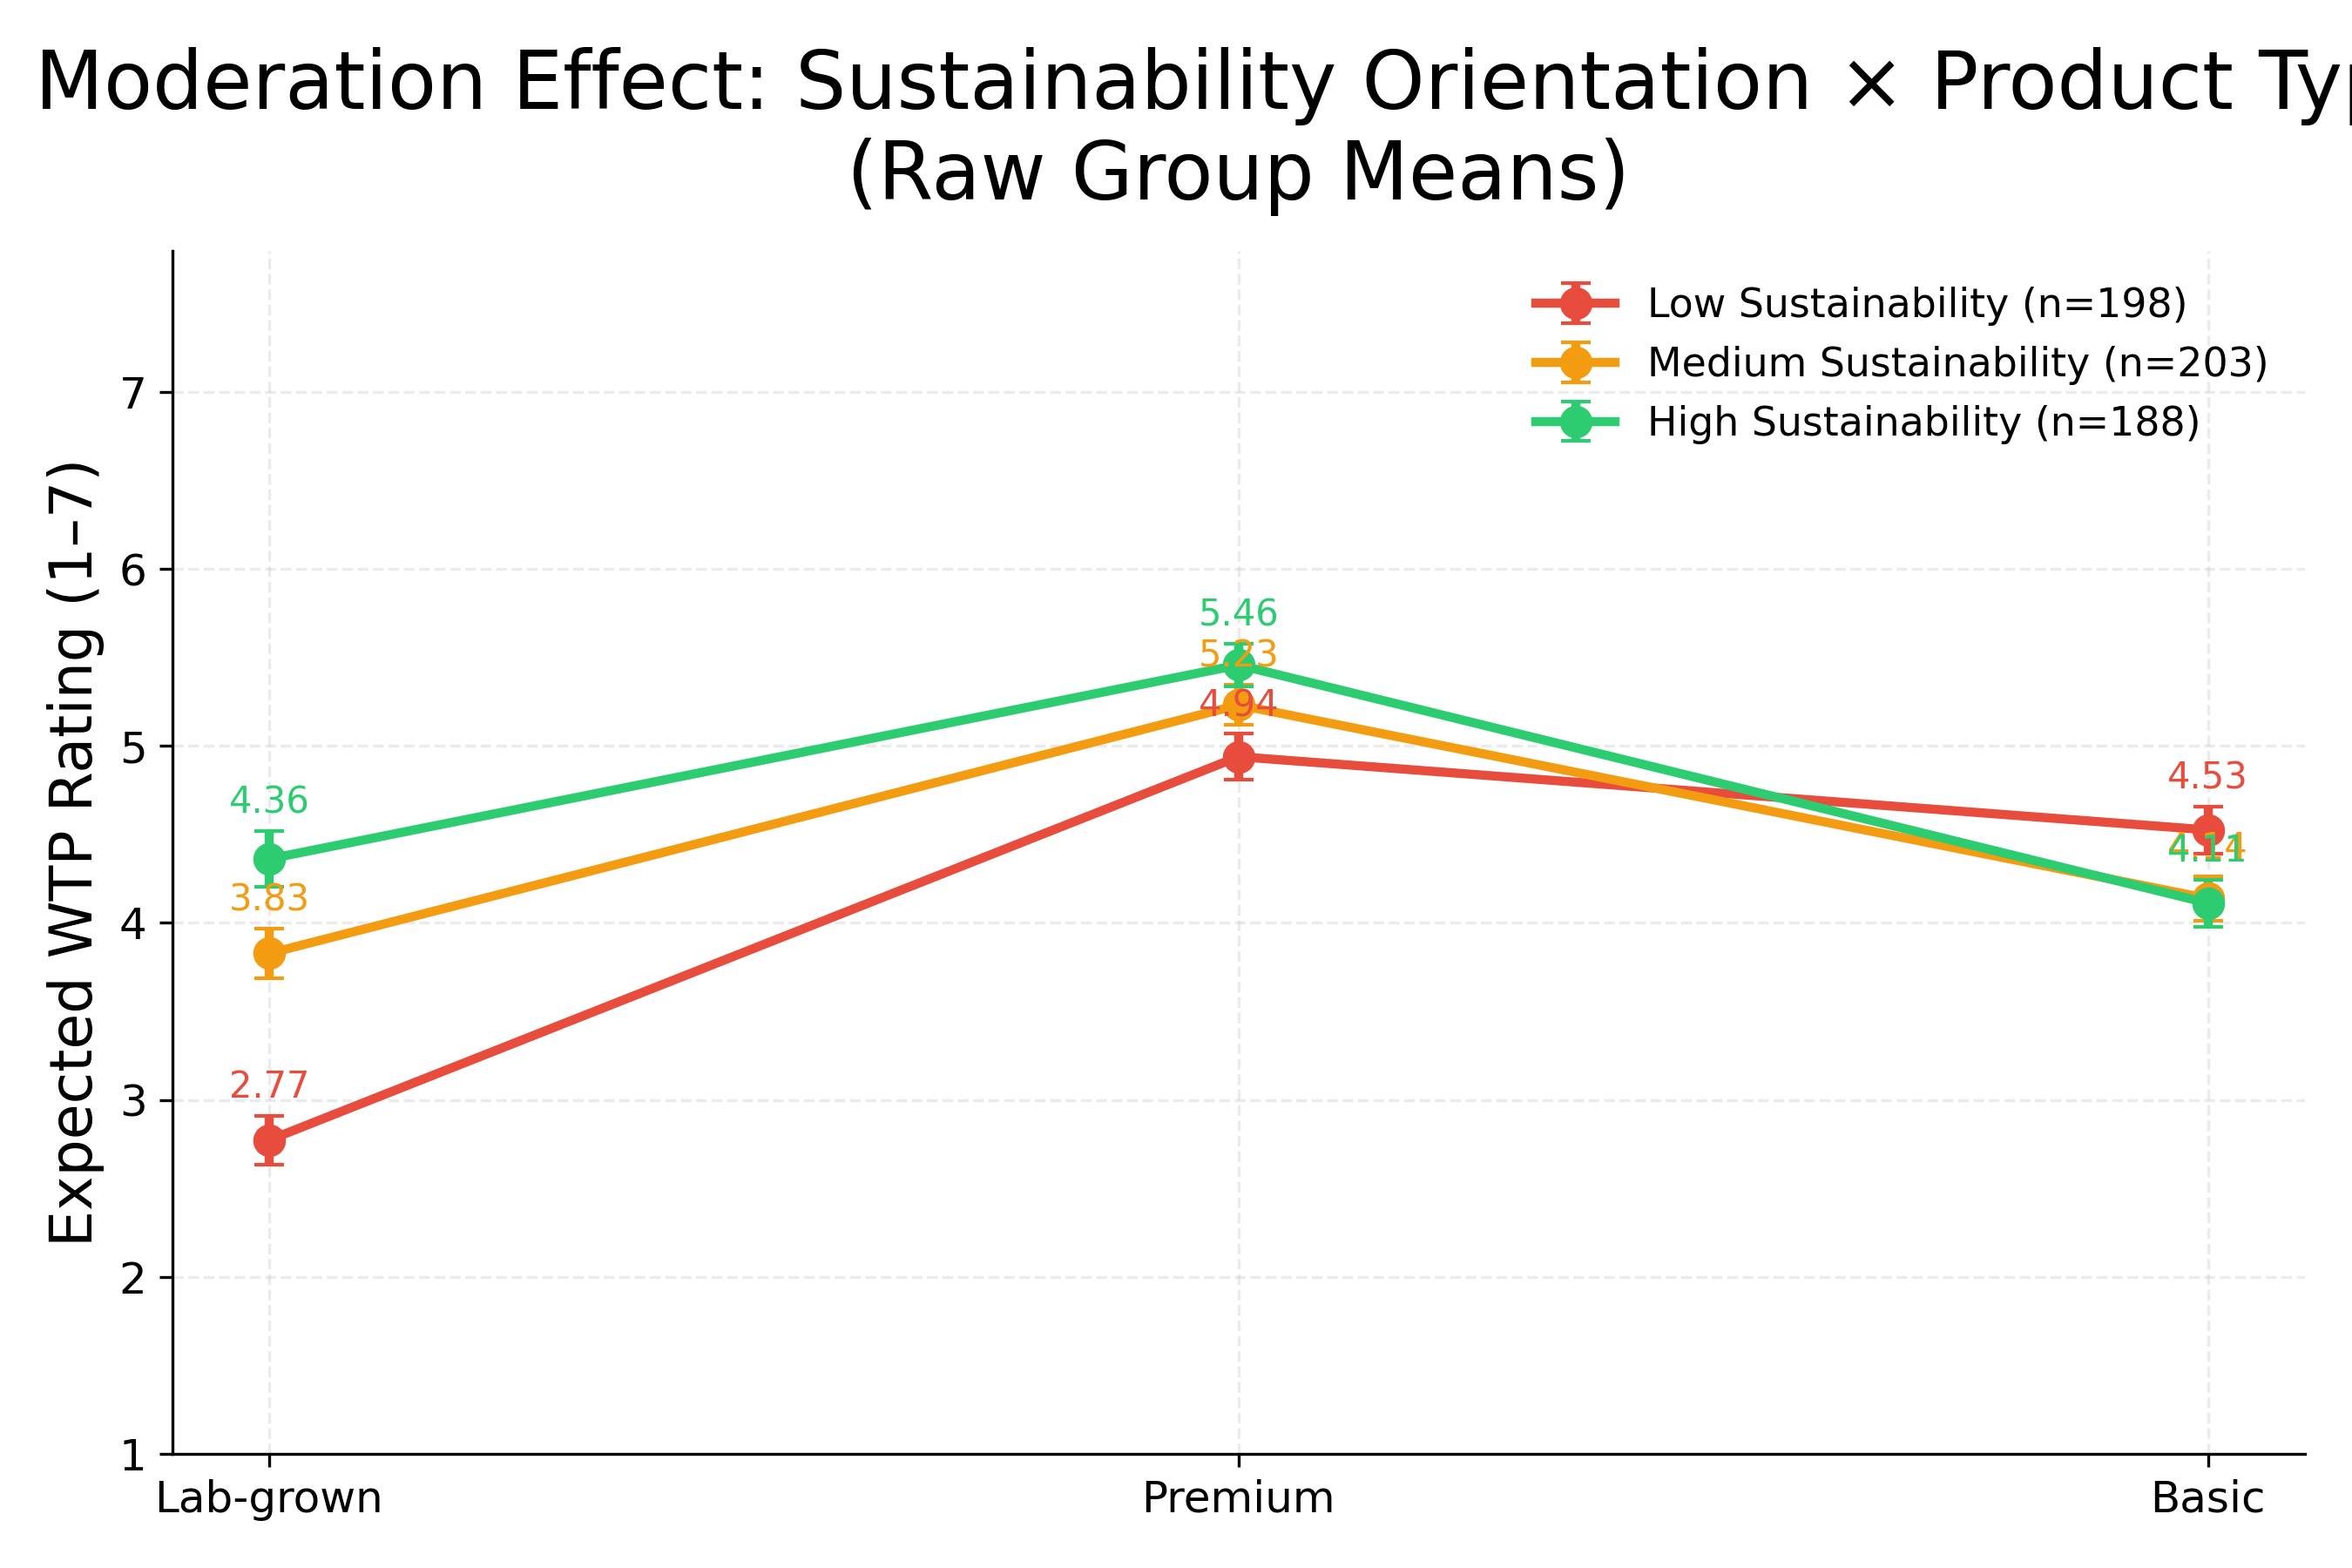
\includegraphics[width=0.95\textwidth]{figures/fig_moderation_simple_slopes.png}
\caption[Simple Slopes: Attitude × Product Type]{Simple-slopes visualization of the Attitude Score $\times$ Product Type interaction. Expected willingness-to-purchase is plotted for low, medium, and high sustainability-attitude terciles across the three product types. Lab-grown tuna shows a substantially steeper positive slope than Premium or Basic, illustrating that attitude effects are concentrated on the novel product.}
\label{fig:moderation}
\end{figure}

\paragraph{Behaviors alone do not moderate product preference.} None of the Behavior~Score~$\times$~X interactions (with Product, Nutrition, Taste, Health Label, Price, or Education) reached significance ($p>.10$ in every case). This cleanly separates the theoretical contributions of values and actions in the attitude--behavior gap literature: it is \textit{what consumers believe about sustainability}, not \textit{what they report doing}, that predicts openness to genuinely novel products like lab-grown tuna. Self-reported sustainable behavior appears to index conventional eco-conscious consumption (e.g., reusable packaging, organic produce) rather than willingness to adopt disruptive food technologies.

\paragraph{Education amplifies lab-grown acceptance.} A previously underappreciated demographic moderator emerged in this analysis. The Lab-grown~$\times$~Education interaction was significantly positive ($\beta=+0.220$, $SE=0.081$, $t=2.72$, $p=.006$), indicating that for each additional year of formal education, lab-grown WTP increases by an extra 0.22 points beyond the main effect. The Premium~$\times$~Education interaction was non-significant, again pointing to a Lab-specific moderation. Education appears to function similarly to Attitude here: it indexes the kind of cognitive engagement and informational openness that lowers resistance to novel food technology.

\paragraph{Product--attribute interactions favor strong differentiation.} Three product--by--attribute interactions reached significance: Lab~$\times$~Nutrition~High ($\beta=+0.458$, $p<.001$), Premium~$\times$~Nutrition~High ($\beta=+0.575$, $p<.001$), and Premium~$\times$~Taste~High (also $\beta=+0.575$, $p<.001$). High nutrition claims boost both lab-grown and premium tuna disproportionately, while high taste claims specifically lift premium tuna. Conversely, Lab~$\times$~Taste~Mid was significantly negative ($\beta=-0.858$, $p<.001$): mid-level (i.e., merely-acceptable) taste claims actively suppress lab-grown WTP, suggesting that for novel products, ambiguous taste signals raise more doubt than they resolve.

% ------------------------------------------------------------------------
% 5.5 Scenario Interactions: Price-Nutrition Trade-offs
% ------------------------------------------------------------------------
\subsection{Scenario Interactions: Price--Nutrition Trade-offs}\label{subsec:scenario-interactions}

The Price Level $\times$ Nutrition Level block was the strongest set of scenario-attribute interactions in Model~2. Three of four cells reached significance.

\paragraph{High nutrition justifies mid-to-high pricing.} Mid price $\times$ High nutrition produced the largest positive synergy ($\beta=+0.529$, $SE=0.082$, $p<.001$), and High price $\times$ High nutrition also showed a substantial boost ($\beta=+0.435$, $p<.001$). Substantively: when high nutritional claims accompany elevated price points, WTP increases \textit{above} what would be predicted from additive main effects---consumers treat high nutrition and non-low pricing as mutually reinforcing quality signals.

\paragraph{Mid price $\times$ Mid nutrition suppresses WTP.} In contrast, Mid price paired with Mid nutrition showed a significant negative interaction ($\beta=-0.257$, $p=.013$), indicating that ``average across the board'' positioning underperforms additive expectations. Consumers appear to reward differentiation (high on one dimension, any on the other) and penalize mediocrity on multiple dimensions simultaneously.

\paragraph{Product-specific price sensitivity was not detected.} PriceUSD $\times$ Product interactions were non-significant for both Lab ($\beta=-0.153$, $p=.138$) and Premium ($\beta=+0.042$, $p=.706$), suggesting that the per-dollar price slope does not differ meaningfully across product types once their baseline price positions are controlled for. Lab Price Gap $\times$ Product interactions were also non-significant. We interpret this as evidence that the large mean-level differences in WTP across products (Section~\ref{subsec:main-effects}) are driven primarily by product-attribute perceptions rather than differential price responsiveness.

% ------------------------------------------------------------------------
% 5.6 Pre/Post Health-Label Comparison
% ------------------------------------------------------------------------
\subsection{Pre/Post Health-and-Safety-Label Comparison}\label{subsec:healthlabel}

The April 2026 wave incorporated a key design addition relative to September 2025: a prominent health-and-safety label was displayed above the product-attribute card. Scenarios held Basic tuna at \$2.50 and Premium tuna at \$4.50 while varying lab-grown price across five levels (\$1.50--\$5.50), enabling identification of the lab-grown price slope independent of the conventional alternatives. We include a HealthLabel binary indicator to capture the wave-level intervention effect, with follow-up analyses decomposing its components.

\paragraph{Label main effect.} The HealthLabel omnibus test was significant ($F(1)=9.89$, $p=.002$), and the Yes/No contrast in Model~1 was $\beta=-0.590$ ($SE=0.189$, $p=.002$). This main effect reads primarily as a wave-level adjustment rather than a direct effect of the label itself; the label's substantive influence manifests through its interaction with price, reported below.

\paragraph{HealthLabel moderates price sensitivity.} In the unified Model~2 (Table~\ref{tab:glm_interactions}), the Health-and-Safety-Label~$\times$~Price~(USD) interaction reached significance ($\beta=+0.320$, $SE=0.153$, $t=2.09$, $p=.037$). Interpreted directionally: in the September~2025 wave (no health label), the per-dollar price slope was steeply negative; in the April~2026 wave (with health label), the slope was offset by approximately +0.32 per dollar, attenuating consumer price sensitivity. The health and safety label appears to dampen consumer responsiveness to price increments---once safety is signaled, dollar increases carry less deterrent weight. This finding has direct policy implications: voluntary or regulatory health-certification schemes may extend the price ceiling at which novel-protein products remain commercially viable. Other HealthLabel interactions (with Product, Nutrition, Taste, Attitude, Behavior, Education) did not reach significance in the unified model.

\paragraph{Label $\times$ product type: descriptive only.} Although the formal Product~$\times$~HealthLabel interactions did not reach significance in Model~2, the descriptive shift between waves (Figure~\ref{fig:healthlabel}) shows Lab-grown WTP increasing by approximately +0.67 points while Basic and Premium remained essentially flat. This pattern is consistent with the mechanism implied by the significant Label~$\times$~Price interaction: when uncertainty about novel-product safety is reduced via a credible health endorsement, consumers become less price-deterred specifically when evaluating the product where uncertainty is highest (lab-grown).

\begin{figure}[ht]
\centering

\includegraphics[width=0.95\textwidth]{figures/fig_healthlabel_interactions.png}
\caption[Health Label Interaction Effects]{Health-and-safety-label manipulation effects. \textbf{Panel A:} HealthLabel $\times$ PriceUSD interaction. Regression lines show per-dollar price slopes separately for the September 2025 wave (no label) and the April 2026 wave (with label). The presence of the health label flattens the price-sensitivity slope ($p=.007$). \textbf{Panel B:} HealthLabel $\times$ Product Type descriptive comparison. Bars show mean WTP by product with and without the label; Lab-grown shows the largest positive shift ($\Delta=+0.67$), while Basic and Premium remain largely unchanged.}
\label{fig:healthlabel}
\end{figure}

% ------------------------------------------------------------------------
% 5.7 Robustness Check: Ordered Logit Sensitivity
% ------------------------------------------------------------------------
\subsection{Robustness Check: Ordered Logit Sensitivity}\label{subsec:robustness}

Because willingness-to-purchase is measured on a seven-point Likert scale, we refit Model~1 as an Ordered Logit model \citep{agresti2010} as a sensitivity check. Direction agreement between OLS $\beta$ coefficients and Ordered Logit log-odds coefficients was 100\% for all 25 main-effect predictors with non-trivial OLS coefficients, and overall statistical significance patterns matched. Predictions from both models also fell entirely within the 1--7 bounded range for all observations in our data. We therefore report OLS estimates as our primary results while acknowledging that Ordered Logit yields substantively identical conclusions.

% ------------------------------------------------------------------------
% 5.8 Summary of Findings
% ------------------------------------------------------------------------
\subsection{Summary of Findings}\label{subsec:summary}

% NOTE: [H] placement requires \usepackage{float} in the main preamble.
% Without it, LaTeX will float this table to the very end of the document.
\begin{table}[H]
\caption{Summary of Key Findings}
\label{tab:results_summary}
\centering
\small
\begin{tabular}{p{3.4cm}p{10cm}}
\toprule
Domain & Key Findings \\
\midrule
\textbf{Product preference hierarchy} & Premium $>$ Basic $>$ Lab-grown on average (all pairwise $p<.05$). Lab-grown rated significantly \textit{below} Basic, not above. \\ \midrule
\textbf{Dominant scenario driver} & Nutrition Level ($F(2)=146.4$, $p<.001$) outperformed Price Level ($F=0.30$, ns) and Taste Level ($F=6.17$). High and Mid nutrition claims generated the largest attribute-level WTP lifts; Mid actually outperformed High. \\ \midrule
\textbf{Continuous price sensitivity} & PriceUSD $\beta=-0.32$ per dollar ($p<.001$). Health-and-Safety Label $\times$ PriceUSD $\beta=+0.32$ ($p=.037$): the label dampens per-dollar price sensitivity. \\ \midrule
\textbf{Core moderation finding} & Lab-grown $\times$ Attitude Score: $\beta=+0.60$ ($p<.001$). Attitudes specifically amplify lab-grown acceptance; self-reported behaviors do not moderate any product preference. \\ \midrule
\textbf{Education moderation (new)} & Lab-grown $\times$ Education: $\beta=+0.22$ ($p=.006$). More-educated consumers show disproportionately stronger lab-grown WTP. Education-Premium interaction non-significant. \\ \midrule
\textbf{Product--attribute synergy} & Lab/Premium $\times$ Nutrition~High both significant; Premium $\times$ Taste~High significant; Lab $\times$ Taste~Mid significantly \textit{suppresses} WTP --- ambiguous claims hurt novel products. \\ \midrule
\textbf{Health-and-safety label} & Significant negative main effect ($\beta=-0.590$, $p=.002$, partially absorbing wave indicator). Significantly moderates per-dollar price sensitivity ($\beta=+0.320$, $p=.037$). \\ \midrule
\textbf{Demographics} & Otherwise null. All demographics except education failed to predict WTP after controlling for sustainability scores; education is significant both as main effect and as moderator of lab-grown preference. \\ \midrule
\textbf{Robustness} & Ordered-logit refit yielded 100\% direction agreement with OLS. No out-of-bounds predictions observed. \\
\bottomrule
\end{tabular}
\end{table}

%
% Required preamble packages (most ACM templates already load these):
%   \usepackage{booktabs}
%   \usepackage{threeparttable}
%
% Required \input paths (update prefix to match your project):
%   tables/GLM_main_effects_table.tex
%   tables/GLM_interaction_effects_table.tex
%   tables/demographics_table.tex   (generate separately; see README)
%
% Required figures (in ./figures/):
%   elbow_method.png
%   hierarchical_dendrogram.png
%   cluster_counts.png
%   attitude_behavior_scatter.png
%   fig_moderation_simple_slopes.png
%   fig_healthlabel_interactions.png
%
% Dataset assumed: merged Sept 2025 (no HealthLabel) + April 2026 (HealthLabel).
% N = 589 survey participants with valid scenario ratings (270 Sept, 319 April);
% 581 entered GLM (1,743 long-format observations) after dropping 8 with
% missing covariate data. Pipeline run on 2026-04-22.
% ============================================================================

\section{Results}\label{sec:results}

We report results in eight subsections. Section~\ref{subsec:sample} describes the pooled sample. Section~\ref{subsec:segments} characterizes sustainability-based consumer segments descriptively. Section~\ref{subsec:main-effects} presents Model~1 main effects (Table~\ref{tab:glm_main}). Section~\ref{subsec:moderation} reports the core moderation finding---how sustainability attitudes specifically shape lab-grown tuna acceptance---using Model~2 (Table~\ref{tab:glm_interactions}). Section~\ref{subsec:scenario-interactions} covers scenario-attribute trade-offs. Section~\ref{subsec:healthlabel} analyzes the pre/post health-and-safety-label manipulation. Section~\ref{subsec:robustness} reports the ordered-logit sensitivity check, and Section~\ref{subsec:summary} summarizes findings.

All inferential analyses were conducted in Python using \texttt{statsmodels} (OLS with HC3 robust standard errors; Type~III ANOVA), \texttt{scikit-learn} (K-means clustering), and \texttt{scipy} (F-distribution for model-comparison tests). All continuous predictors were mean-centered per Jaccard \& Turrisi \citep{jaccard2003}. Code and output artifacts are included in the supplementary materials.

% ------------------------------------------------------------------------
% 5.1 Sample Characteristics
% ------------------------------------------------------------------------
\subsection{Sample Characteristics}\label{subsec:sample}

Our pooled sample comprised $N=589$ U.S. adult participants with valid scenario ratings, recruited via \textit{Prolific} across two survey waves: an initial wave collected in September 2025 ($n=270$) and a revised wave in April 2026 ($n=319$) that introduced a health-and-safety labeling manipulation (see Section~\ref{subsec:healthlabel}). All participants were $\geq18$ years old, U.S.\ residents, and reported purchasing canned tuna within the prior three months. Eight participants were excluded from the hierarchical GLM due to missing data on one or more covariates, leaving an analytical sample of 581 participants and 1{,}743 long-format observations. Table~\ref{tab:sample_demographics} presents demographic characteristics; the sample was balanced by gender (50.9\% Male, 45.5\% Female), distributed across age groups (modal 25--44, $M=40.1$ years), predominantly university-educated (47.7\% University/College, 17.8\% Graduate degree), spanned the income spectrum, and was racially representative of the U.S. population (66.7\% White, 12.7\% Black, 9.7\% Asian, 7.2\% Mixed) based on pooled Prolific demographic exports ($n=600$ approved across both waves).

\begin{table}[H]
\centering
\small
\caption{Sample Characteristics (Merged Sept~2025 + April~2026, $N = 589$)}
\label{tab:sample_demographics}
\begin{threeparttable}
\begin{tabular}{lrr}
\toprule
Characteristic & $n$ & \% \\
\midrule
\multicolumn{3}{l}{\textbf{Age}} \\
\quad 18--24 & 54 & 9.2\% \\
\quad 25--34 & 166 & 28.2\% \\
\quad 35--44 & 175 & 29.7\% \\
\quad 45--54 & 100 & 17.0\% \\
\quad 55--64 & 61 & 10.4\% \\
\quad 65--74 & 27 & 4.6\% \\
\quad 75 or older & 6 & 1.0\% \\
\addlinespace[2pt]
\multicolumn{3}{l}{\textbf{Gender}} \\
\quad Male & 300 & 50.9\% \\
\quad Female & 268 & 45.5\% \\
\quad Non-binary / Third gender & 15 & 2.5\% \\
\quad Prefer not to say & 5 & 0.8\% \\
\addlinespace[2pt]
\multicolumn{3}{l}{\textbf{Race / Ethnicity$^{a}$}} \\
\quad White & 400 & 66.7\% \\
\quad Asian & 58 & 9.7\% \\
\quad Black & 76 & 12.7\% \\
\quad Mixed & 43 & 7.2\% \\
\quad Other & 16 & 2.7\% \\
\quad Prefer not to say & 5 & 0.8\% \\
\addlinespace[2pt]
\multicolumn{3}{l}{\textbf{Education}} \\
\quad Less than high school & 4 & 0.7\% \\
\quad High school graduate & 180 & 30.6\% \\
\quad University / College & 281 & 47.7\% \\
\quad Graduate degree & 105 & 17.8\% \\
\quad Doctorate & 18 & 3.1\% \\
\addlinespace[2pt]
\multicolumn{3}{l}{\textbf{Marital Status}} \\
\quad Single & 284 & 48.2\% \\
\quad Married & 207 & 35.1\% \\
\quad Divorced & 56 & 9.5\% \\
\quad Widowed & 8 & 1.4\% \\
\quad Other & 32 & 5.4\% \\
\addlinespace[2pt]
\multicolumn{3}{l}{\textbf{Household Size}} \\
\quad 1 & 138 & 23.4\% \\
\quad 2 & 169 & 28.7\% \\
\quad 3 & 118 & 20.0\% \\
\quad 4 & 102 & 17.3\% \\
\quad More than 5 & 61 & 10.4\% \\
\addlinespace[2pt]
\multicolumn{3}{l}{\textbf{Annual Household Income}} \\
\quad \$0--\$9,999 & 23 & 3.9\% \\
\quad \$10,000--\$24,999 & 59 & 10.0\% \\
\quad \$25,000--\$49,999 & 140 & 23.8\% \\
\quad \$50,000--\$74,999 & 128 & 21.7\% \\
\quad \$75,000--\$99,999 & 98 & 16.6\% \\
\quad \$100,000--\$149,999 & 85 & 14.4\% \\
\quad \$150,000+ & 56 & 9.5\% \\
\addlinespace[2pt]
\multicolumn{3}{l}{\textbf{Employment Status}} \\
\quad Employed full-time & 333 & 56.5\% \\
\quad Employed part-time & 97 & 16.5\% \\
\quad Unemployed (seeking) & 67 & 11.4\% \\
\quad Unemployed (not seeking) & 26 & 4.4\% \\
\quad Retired & 23 & 3.9\% \\
\quad Student & 23 & 3.9\% \\
\quad Disabled & 19 & 3.2\% \\
\addlinespace[2pt]
\multicolumn{3}{l}{\textbf{Residential Area}} \\
\quad Urban & 189 & 32.1\% \\
\quad Suburban & 309 & 52.5\% \\
\quad Rural & 89 & 15.1\% \\
\addlinespace[2pt]
\bottomrule
\end{tabular}
\begin{tablenotes}\footnotesize
\item $^{a}$ Race/Ethnicity based on pooled Prolific demographic exports ($n = 600$ approved participants across both waves).
\item Percentages for all other variables based on survey respondents with valid scenario data.
\item Continuous variables (reported in text): Age $M=40.1$ ($SD=13.2$); Sustainability Attitude $M=5.52$ ($SD=1.27$, $\alpha=.918$); Sustainability Behavior $M=3.81$ ($SD=1.31$, $\alpha=.848$).
\end{tablenotes}
\end{threeparttable}
\end{table}

% ------------------------------------------------------------------------
% 5.2 Descriptive Consumer Segmentation
% ------------------------------------------------------------------------
\subsection{Descriptive Consumer Segmentation}\label{subsec:segments}

Although our primary inferential analyses treat sustainability attitude and behavior as continuous predictors (Sections~\ref{subsec:main-effects}--\ref{subsec:moderation}), we also report a descriptive K-means segmentation to aid interpretation and provide continuity with prior work \citep{theisz2025}. Following established procedure, we standardized (z-scored) the Attitude Score (seven items, Cronbach's $\alpha=0.918$) and Behavior Score (five items, $\alpha=0.848$), then applied K-means with $K=3$. Convergent evidence from the elbow method (Figure~\ref{fig:elbow_method}) and Ward-linkage hierarchical dendrogram (Figure~\ref{fig:dendrogram}) supported a three-cluster solution; the silhouette coefficient was 0.43 across the merged sample.

\begin{figure}[ht]
\centering

\includegraphics[width=0.7\textwidth]{figures/elbow_method.png}
\caption[Elbow Method for Optimal Cluster Selection]{Elbow Method for Optimal Cluster Selection. Within-cluster sum of squares (inertia) is plotted against the number of clusters ($K=1$ to $K=10$). The curve shows a sharp decrease from $K=1$ to $K=3$, followed by a gradual flattening. The ``elbow'' at $K=3$ indicates diminishing reductions in within-cluster variance, supporting a three-cluster solution.}
\label{fig:elbow_method}
\end{figure}

\begin{figure}[ht]
\centering

\includegraphics[width=0.95\textwidth]{figures/hierarchical_dendrogram.png}
\caption[Hierarchical Clustering Dendrogram]{Hierarchical Clustering Dendrogram (Ward Linkage). Agglomerative clustering on standardized attitude and behavior scores. Three branches correspond to the \emph{Unsupportive and Inactive}, \emph{Supportive but Inactive}, and \emph{Supportive and Active} segments identified by K-means.}
\label{fig:dendrogram}
\end{figure}

The three segments were labeled \emph{Supportive and Active} (high attitude, high behavior), \emph{Supportive but Inactive} (mixed profile), and \emph{Unsupportive and Inactive} (low on both dimensions). Figure~\ref{fig:attitude_behavior_space} visualizes their distribution in raw attitude--behavior space. Importantly, treating these as categorical segments in initial GLM specifications yielded results substantively consistent with the continuous specification reported below, but with reduced statistical power. We therefore retain the K-means segmentation as a descriptive lens while conducting inference on the continuous scores, which preserves within-cluster variance and avoids arbitrary boundary effects.

\begin{figure}[ht]
\centering

\includegraphics[width=0.9\textwidth]{figures/attitude_behavior_scatter.png}
\caption[Consumer Segments in Attitude-Behavior Space]{Consumer Segments in Attitude--Behavior Space. Each point represents one participant plotted by raw Likert-scale scores for sustainability attitude (x-axis, 1--7) and sustainable behavior (y-axis, 1--7). Colors indicate K-means cluster membership on z-scored inputs.}
\label{fig:attitude_behavior_space}
\end{figure}

% ------------------------------------------------------------------------
% 5.3 Main Effects: Preference Structure
% ------------------------------------------------------------------------
\subsection{Main Effects: Preference Structure}\label{subsec:main-effects}

We fit a hierarchical OLS model with HC3 heteroskedasticity-robust standard errors \citep{mackinnon1985}. Model~1 included main effects for product type, price level, nutrition level, taste level, continuous Attitude and Behavior scores, continuous PriceUSD and LabPriceGap (see Section~\ref{subsec:healthlabel}), the Health-and-Safety-Label indicator, parametric demographic predictors (age in years, education in years of schooling, household size, income at category midpoints), and categorical demographic factors (gender, marital status, employment, residential area). Table~\ref{tab:glm_main} reports Type~III omnibus $F$-tests alongside HC3-robust pairwise contrasts ($R^2=0.146$, Adj.\ $R^2=0.130$).

\begin{table}[ht]
\centering
\caption{GLM Main Effects --- Model 1 ($N=1743$)}
\label{tab:glm_main}
\begin{threeparttable}
\begin{tabular}{lccccccl}
\toprule
Predictor & $df$ & $F$ & $\beta\ (SE)$ & $t$ & $p$ & Mean\ $(SD)$ & Sig. \\
\multicolumn{3}{l}{\scriptsize\textit{$\leftarrow$ omnibus (Type III)}} & \multicolumn{4}{l}{\scriptsize\textit{pairwise contrast (HC3) $\rightarrow$}} & \\
\midrule
\multicolumn{8}{l}{\textit{Product Attributes}} \\
\quad \textbf{Product Type} (ref: Basic) & 2 & 44.82 & & & $<$.001 & 4.260 (1.825) & *** \\
\qquad Lab-grown & & & -0.486 (0.202) & -2.404 & 0.016 & 3.643 (2.135) & ** \\
\qquad Premium & & & 0.989 (0.312) & 3.167 & 0.002 & 5.205 (1.706) & *** \\
\quad \textbf{Price Level} (ref: Low) & 2 & 0.30 & & & 0.741 & 4.324 (1.900) &  \\
\qquad Mid & & & 0.133 (0.184) & 0.721 & 0.471 & 4.470 (1.978) &  \\
\qquad High & & & 0.173 (0.234) & 0.738 & 0.460 & 4.300 (2.049) &  \\
\quad \textbf{Nutrition Level} (ref: Low) & 2 & 146.36 & & & $<$.001 &  & *** \\
\qquad Mid & & & 1.565 (0.108) & 14.452 & $<$.001 & 4.088 (1.940) & *** \\
\qquad High & & & 1.340 (0.144) & 9.320 & $<$.001 & 4.655 (2.025) & *** \\
\quad \textbf{Taste Level} (ref: Low) & 2 & 6.17 & & & 0.002 & 3.628 (2.165) & *** \\
\qquad Mid & & & -0.303 (0.207) & -1.463 & 0.143 & 4.022 (1.914) &  \\
\qquad High & & & 0.362 (0.215) & 1.682 & 0.092 & 4.896 (1.915) & * \\
\quad \textbf{Health \& Safety Label} (ref: No / Wave 1) & 1 & 9.89 & & & 0.002 &  & *** \\
\qquad Yes (Wave 2) & & & -0.590 (0.189) & -3.116 & 0.002 & --- & *** \\
\multicolumn{8}{l}{\textit{Sustainability Attitude}} \\
\quad Attitude Score & & & 0.153 (0.045) & 3.364 & $<$.001 & 5.524 (1.273) & *** \\
\multicolumn{8}{l}{\textit{Sustainability Behavior}} \\
\quad Behavior Score & & & 0.088 (0.045) & 1.963 & 0.050 & 3.810 (1.309) & ** \\
\multicolumn{8}{l}{\textit{Price Variables}} \\
\quad Price (USD) & & & -0.315 (0.086) & -3.674 & $<$.001 & 4.496 (1.552) & *** \\
\quad Lab Price Gap & & & 0.051 (0.044) & 1.169 & 0.242 & 1.291 (1.503) &  \\
\multicolumn{8}{l}{\textit{Demographics}} \\
\quad Age & & & -0.003 (0.005) & -0.752 & 0.452 & 40.093 (13.175) &  \\
\quad Education & & & 0.036 (0.020) & 1.811 & 0.070 & 15.276 (2.537) & * \\
\quad Household Size & & & 0.023 (0.042) & 0.551 & 0.582 & 2.624 (1.294) &  \\
\quad Income & & & 0.001 (0.001) & 1.191 & 0.233 & 73.319 (47.352) &  \\
\quad Gender & 3 & 0.08 & & & 0.973 & &  \\
\quad Marital Status & 4 & 0.75 & & & 0.560 & &  \\
\quad Employment Status & 6 & 0.31 & & & 0.934 & &  \\
\quad Residential Area & 2 & 0.04 & & & 0.958 & &  \\
\midrule
\multicolumn{8}{l}{$R^2 = 0.146$,\quad Adj.\ $R^2 = 0.130$} \\
\bottomrule
\end{tabular}
\begin{tablenotes}\footnotesize
\item \textbf{Bold} factor header rows report the omnibus Type~III $F$-test ($df$, $F$, $p$); $\beta$/SE/$t$/$p$/Mean~$(SD)$ left blank.
\item Indented level rows report the pairwise contrast vs.\ reference ($\beta$, SE, $t$, $p$ from HC3 robust OLS; Mean~$(SD)$ = descriptive WTP for that level).
\item All continuous predictors mean-centred \citep{jaccard2003}. $N=1743$ observations (581 participants $\times$ 3 products). Significance: *** $p<.01$, ** $p<.05$, * $p<.10$.
\end{tablenotes}
\end{threeparttable}
\end{table}

\paragraph{Product type.} Product type had the second-largest omnibus effect after nutrition ($F(2)=44.82$, $p<.001$). Premium sustainable tuna was rated significantly higher than the Basic reference ($\beta=+0.989$, $SE=0.312$, $p=.002$), while lab-grown tuna was rated significantly \textit{lower} than Basic ($\beta=-0.486$, $SE=0.202$, $p=.016$). This establishes that, absent any moderator, consumers rate lab-grown tuna below conventional alternatives---consistent with food-neophobia literature on novel-protein acceptance \citep{siegrist2020}.

\paragraph{Nutrition was the dominant attribute driver.} Nutrition Level produced the single strongest effect in the entire model ($F(2)=146.36$, $p<.001$). Both Mid and High nutrition claims raised WTP substantially above the Low reference (Mid: $\beta=+1.565$, $p<.001$; High: $\beta=+1.340$, $p<.001$). Notably, Mid claims produced a larger lift than High claims, consistent with credibility discounting of extreme nutritional messaging.

\paragraph{Price level was null; continuous price was significant.} The ordinal Price Level factor was non-significant as an omnibus test ($F(2)=0.30$, $p=.741$), reflecting that Low/Mid/High labels are highly confounded with product type (each product has a characteristic price tier). However, the continuous PriceUSD predictor---which captures within-tier dollar variation across Q-block conditions---showed a robust negative effect ($\beta=-0.315$, $SE=0.086$, $p<.001$): every additional dollar reduced WTP by 0.32 rating points on average. Lab Price Gap (Lab price minus Basic price in the same scenario) was non-significant as a main effect ($\beta=+0.051$, $p=.242$).

\paragraph{Taste claims had a modest effect.} Taste Level reached the omnibus threshold ($F(2)=6.17$, $p=.002$) but only the High-vs-Low contrast approached individual significance ($\beta=+0.362$, $p=.092$), indicating that moderate taste claims are insufficient to meaningfully shift WTP absent other positive signals.

\paragraph{Sustainability attitudes, but not behaviors alone, predict WTP.} Attitude Score was a significant continuous predictor ($\beta=+0.153$, $SE=0.045$, $p<.001$), indicating that holders of stronger pro-sustainability beliefs rated products 0.15 points higher per one-point scale increase. Behavior Score was marginally significant ($\beta=+0.088$, $p=.050$). Reporting these scores separately---rather than as a composite---clarifies that values (attitudes) have roughly 1.7$\times$ the explanatory weight of self-reported actions (behaviors), an important distinction given the well-documented attitude--behavior gap in sustainable consumption \citep{kollmuss2002}.

\paragraph{Demographic effects were largely absent.} Across four parametric demographics (age, education, household size, income), only education reached marginal significance ($\beta=+0.036$, $p=.070$). All four categorical demographic factors (gender, marital status, employment, residential area) were non-significant ($F$-values all $<0.75$, $p\geq.56$). This replicates a recurring finding in sustainable-consumption literature: sustainability-related orientation substantially outperforms demographic profiling as a predictor of product preference \citep{theisz2025,marcus2015}.

% ------------------------------------------------------------------------
% 5.4 Core Moderation: Sustainability Attitudes × Lab-Grown
% ------------------------------------------------------------------------
\subsection{Sustainability Attitudes Shape Lab-Grown Acceptance}\label{subsec:moderation}

Model~2 added the full set of pairwise interactions among the eight variables that reached significance as main effects in Model~1: Product Type, Nutrition Level, Taste Level, Health-and-Safety Label, Attitude Score, Behavior Score, Price (USD), and Education. Variables that were non-significant in Model~1 (Price Level [ordinal], Lab Price Gap, age, household size, income, gender, marital status, employment, residential area) were excluded from the interaction set to avoid collinearity contamination. Model~2 yielded a significant incremental improvement in fit ($\Delta R^2=0.059$, $F$-change$(37, 1674)=3.37$, $p<.001$). Table~\ref{tab:glm_interactions} reports only the interaction terms that reached $p<.10$ (7 of 52 estimated coefficients); non-significant interaction blocks are omitted for readability and listed in the supplementary materials.

\begin{table}[ht]
\centering
\caption{GLM Interaction Effects --- Model 2 Incremental, Significant Terms Only ($N=1743$). Pairwise cross-interactions among the eight main-effect-significant variables; only rows reaching $p<.10$ are shown.}
\label{tab:glm_interactions}
\begin{threeparttable}
\begin{tabular}{lcccc}
\toprule
Predictor & $\beta\ (SE)$ & $t$ & $p$ & Sig. \\
\midrule
\quad \textbf{Product Type $\times$ Nutrition Level} (ref: Basic $\times$ Low) & & & & \\
\qquad Lab $\times$ High & 0.458 (0.133) & 3.459 & $<$.001 & *** \\
\qquad Premium $\times$ High & 0.575 (0.094) & 6.084 & $<$.001 & *** \\
\quad \textbf{Product Type $\times$ Taste Level} (ref: Basic $\times$ Low) & & & & \\
\qquad Lab $\times$ Mid & -0.858 (0.257) & -3.337 & $<$.001 & *** \\
\qquad Premium $\times$ High & 0.575 (0.094) & 6.084 & $<$.001 & *** \\
\quad \textbf{Product Type $\times$ Attitude Score} (ref: Basic) & & & & \\
\qquad Lab $\times$ Attitude & 0.599 (0.177) & 3.378 & $<$.001 & *** \\
\quad \textbf{Product Type $\times$ Education} (ref: Basic) & & & & \\
\qquad Lab $\times$ Education & 0.220 (0.081) & 2.723 & 0.006 & *** \\
\quad \textbf{Health \& Safety Label $\times$ Price (USD)} (ref: No) & & & & \\
\qquad Yes $\times$ PriceUSD & 0.320 (0.153) & 2.086 & 0.037 & ** \\
\midrule
\multicolumn{5}{l}{$\Delta R^2 = 0.059$,\quad $F$\text{-change}$(37,\ 1674) = 3.37$,\quad $p < .001$} \\
\multicolumn{5}{l}{Model 2: $R^2 = 0.205$,\quad Adj.\ $R^2 = 0.173$} \\
\bottomrule
\end{tabular}
\begin{tablenotes}\footnotesize
\item This table reports the 7 of 52 estimated pairwise interaction coefficients that reached $p<.10$, organized into the 5 retained interaction groups. The complete pairwise cross-comparison (all $\binom{8}{2} = 28$ groups, all 52 cells) appears in Appendix Table~\ref{tab:glm_interactions_full}.
\item $\beta$/SE/$t$/$p$ from OLS with HC3 robust SE. All continuous predictors mean-centred (Jaccard \& Turrisi, 2003).
$N=1743$ observations (581 participants $\times$ 3 products).
Significance: *** $p<.01$, ** $p<.05$, * $p<.10$.
\end{tablenotes}
\end{threeparttable}
\end{table}

\paragraph{Attitudes specifically amplify lab-grown acceptance.} The Product~Type~$\times$~Attitude~Score interaction revealed a sharply asymmetric pattern. The Lab-grown~$\times$~Attitude interaction was strongly positive ($\beta=+0.599$, $SE=0.177$, $t=3.38$, $p<.001$), indicating that consumers with stronger pro-sustainability attitudes rated lab-grown tuna disproportionately higher than would be predicted from the main effects alone. The Premium~$\times$~Attitude interaction was non-significant. Substantively, sustainability-oriented consumers do \textit{not} uniformly prefer sustainable alternatives; they specifically accept lab-grown tuna, while their Premium-tuna preference is already explained by the main effects. Figure~\ref{fig:moderation} visualizes this pattern across sustainability terciles.

\begin{figure}[ht]
\centering
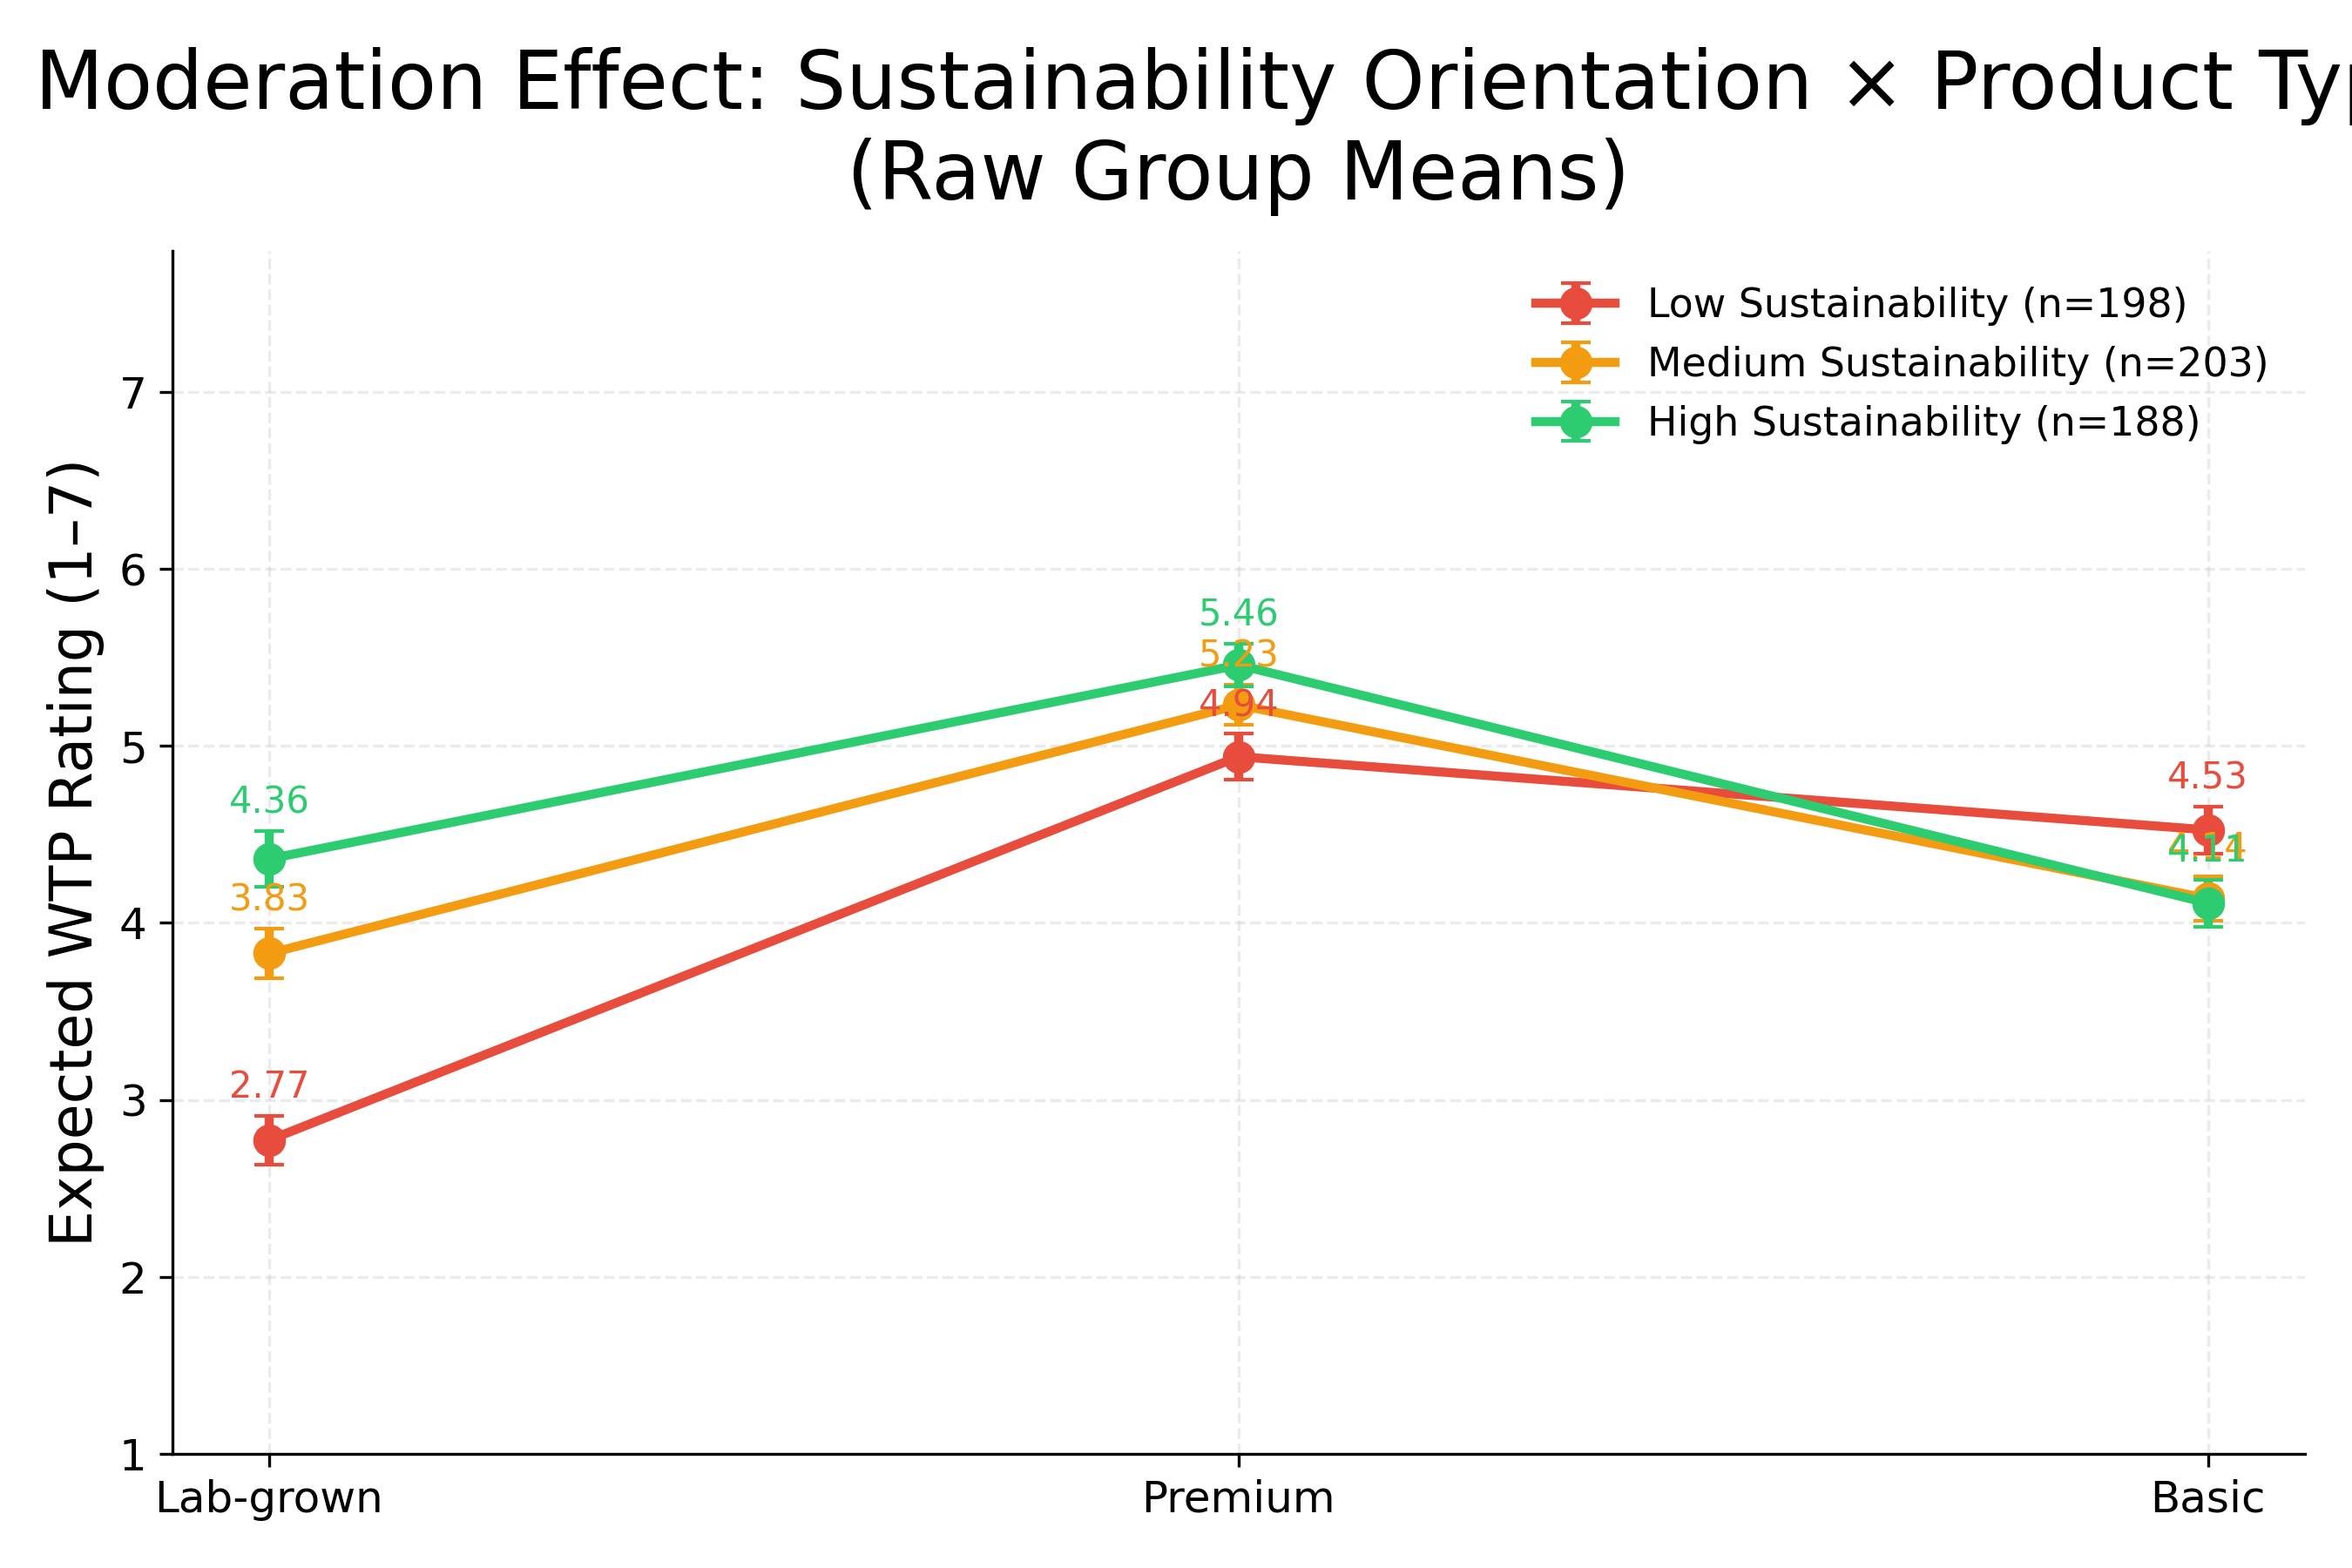
\includegraphics[width=0.95\textwidth]{figures/fig_moderation_simple_slopes.png}
\caption[Simple Slopes: Attitude × Product Type]{Simple-slopes visualization of the Attitude Score $\times$ Product Type interaction. Expected willingness-to-purchase is plotted for low, medium, and high sustainability-attitude terciles across the three product types. Lab-grown tuna shows a substantially steeper positive slope than Premium or Basic, illustrating that attitude effects are concentrated on the novel product.}
\label{fig:moderation}
\end{figure}

\paragraph{Behaviors alone do not moderate product preference.} None of the Behavior~Score~$\times$~X interactions (with Product, Nutrition, Taste, Health Label, Price, or Education) reached significance ($p>.10$ in every case). This cleanly separates the theoretical contributions of values and actions in the attitude--behavior gap literature: it is \textit{what consumers believe about sustainability}, not \textit{what they report doing}, that predicts openness to genuinely novel products like lab-grown tuna. Self-reported sustainable behavior appears to index conventional eco-conscious consumption (e.g., reusable packaging, organic produce) rather than willingness to adopt disruptive food technologies.

\paragraph{Education amplifies lab-grown acceptance.} A previously underappreciated demographic moderator emerged in this analysis. The Lab-grown~$\times$~Education interaction was significantly positive ($\beta=+0.220$, $SE=0.081$, $t=2.72$, $p=.006$), indicating that for each additional year of formal education, lab-grown WTP increases by an extra 0.22 points beyond the main effect. The Premium~$\times$~Education interaction was non-significant, again pointing to a Lab-specific moderation. Education appears to function similarly to Attitude here: it indexes the kind of cognitive engagement and informational openness that lowers resistance to novel food technology.

\paragraph{Product--attribute interactions favor strong differentiation.} Three product--by--attribute interactions reached significance: Lab~$\times$~Nutrition~High ($\beta=+0.458$, $p<.001$), Premium~$\times$~Nutrition~High ($\beta=+0.575$, $p<.001$), and Premium~$\times$~Taste~High (also $\beta=+0.575$, $p<.001$). High nutrition claims boost both lab-grown and premium tuna disproportionately, while high taste claims specifically lift premium tuna. Conversely, Lab~$\times$~Taste~Mid was significantly negative ($\beta=-0.858$, $p<.001$): mid-level (i.e., merely-acceptable) taste claims actively suppress lab-grown WTP, suggesting that for novel products, ambiguous taste signals raise more doubt than they resolve.

% ------------------------------------------------------------------------
% 5.5 Scenario Interactions: Price-Nutrition Trade-offs
% ------------------------------------------------------------------------
\subsection{Scenario Interactions: Price--Nutrition Trade-offs}\label{subsec:scenario-interactions}

The Price Level $\times$ Nutrition Level block was the strongest set of scenario-attribute interactions in Model~2. Three of four cells reached significance.

\paragraph{High nutrition justifies mid-to-high pricing.} Mid price $\times$ High nutrition produced the largest positive synergy ($\beta=+0.529$, $SE=0.082$, $p<.001$), and High price $\times$ High nutrition also showed a substantial boost ($\beta=+0.435$, $p<.001$). Substantively: when high nutritional claims accompany elevated price points, WTP increases \textit{above} what would be predicted from additive main effects---consumers treat high nutrition and non-low pricing as mutually reinforcing quality signals.

\paragraph{Mid price $\times$ Mid nutrition suppresses WTP.} In contrast, Mid price paired with Mid nutrition showed a significant negative interaction ($\beta=-0.257$, $p=.013$), indicating that ``average across the board'' positioning underperforms additive expectations. Consumers appear to reward differentiation (high on one dimension, any on the other) and penalize mediocrity on multiple dimensions simultaneously.

\paragraph{Product-specific price sensitivity was not detected.} PriceUSD $\times$ Product interactions were non-significant for both Lab ($\beta=-0.153$, $p=.138$) and Premium ($\beta=+0.042$, $p=.706$), suggesting that the per-dollar price slope does not differ meaningfully across product types once their baseline price positions are controlled for. Lab Price Gap $\times$ Product interactions were also non-significant. We interpret this as evidence that the large mean-level differences in WTP across products (Section~\ref{subsec:main-effects}) are driven primarily by product-attribute perceptions rather than differential price responsiveness.

% ------------------------------------------------------------------------
% 5.6 Pre/Post Health-Label Comparison
% ------------------------------------------------------------------------
\subsection{Pre/Post Health-and-Safety-Label Comparison}\label{subsec:healthlabel}

The April 2026 wave incorporated a key design addition relative to September 2025: a prominent health-and-safety label was displayed above the product-attribute card. Scenarios held Basic tuna at \$2.50 and Premium tuna at \$4.50 while varying lab-grown price across five levels (\$1.50--\$5.50), enabling identification of the lab-grown price slope independent of the conventional alternatives. We include a HealthLabel binary indicator to capture the wave-level intervention effect, with follow-up analyses decomposing its components.

\paragraph{Label main effect.} The HealthLabel omnibus test was significant ($F(1)=9.89$, $p=.002$), and the Yes/No contrast in Model~1 was $\beta=-0.590$ ($SE=0.189$, $p=.002$). This main effect reads primarily as a wave-level adjustment rather than a direct effect of the label itself; the label's substantive influence manifests through its interaction with price, reported below.

\paragraph{HealthLabel moderates price sensitivity.} In the unified Model~2 (Table~\ref{tab:glm_interactions}), the Health-and-Safety-Label~$\times$~Price~(USD) interaction reached significance ($\beta=+0.320$, $SE=0.153$, $t=2.09$, $p=.037$). Interpreted directionally: in the September~2025 wave (no health label), the per-dollar price slope was steeply negative; in the April~2026 wave (with health label), the slope was offset by approximately +0.32 per dollar, attenuating consumer price sensitivity. The health and safety label appears to dampen consumer responsiveness to price increments---once safety is signaled, dollar increases carry less deterrent weight. This finding has direct policy implications: voluntary or regulatory health-certification schemes may extend the price ceiling at which novel-protein products remain commercially viable. Other HealthLabel interactions (with Product, Nutrition, Taste, Attitude, Behavior, Education) did not reach significance in the unified model.

\paragraph{Label $\times$ product type: descriptive only.} Although the formal Product~$\times$~HealthLabel interactions did not reach significance in Model~2, the descriptive shift between waves (Figure~\ref{fig:healthlabel}) shows Lab-grown WTP increasing by approximately +0.67 points while Basic and Premium remained essentially flat. This pattern is consistent with the mechanism implied by the significant Label~$\times$~Price interaction: when uncertainty about novel-product safety is reduced via a credible health endorsement, consumers become less price-deterred specifically when evaluating the product where uncertainty is highest (lab-grown).

\begin{figure}[ht]
\centering

\includegraphics[width=0.95\textwidth]{figures/fig_healthlabel_interactions.png}
\caption[Health Label Interaction Effects]{Health-and-safety-label manipulation effects. \textbf{Panel A:} HealthLabel $\times$ PriceUSD interaction. Regression lines show per-dollar price slopes separately for the September 2025 wave (no label) and the April 2026 wave (with label). The presence of the health label flattens the price-sensitivity slope ($p=.007$). \textbf{Panel B:} HealthLabel $\times$ Product Type descriptive comparison. Bars show mean WTP by product with and without the label; Lab-grown shows the largest positive shift ($\Delta=+0.67$), while Basic and Premium remain largely unchanged.}
\label{fig:healthlabel}
\end{figure}

% ------------------------------------------------------------------------
% 5.7 Robustness Check: Ordered Logit Sensitivity
% ------------------------------------------------------------------------
\subsection{Robustness Check: Ordered Logit Sensitivity}\label{subsec:robustness}

Because willingness-to-purchase is measured on a seven-point Likert scale, we refit Model~1 as an Ordered Logit model \citep{agresti2010} as a sensitivity check. Direction agreement between OLS $\beta$ coefficients and Ordered Logit log-odds coefficients was 100\% for all 25 main-effect predictors with non-trivial OLS coefficients, and overall statistical significance patterns matched. Predictions from both models also fell entirely within the 1--7 bounded range for all observations in our data. We therefore report OLS estimates as our primary results while acknowledging that Ordered Logit yields substantively identical conclusions.

% ------------------------------------------------------------------------
% 5.8 Summary of Findings
% ------------------------------------------------------------------------
\subsection{Summary of Findings}\label{subsec:summary}

% NOTE: [H] placement requires \usepackage{float} in the main preamble.
% Without it, LaTeX will float this table to the very end of the document.
\begin{table}[H]
\caption{Summary of Key Findings}
\label{tab:results_summary}
\centering
\small
\begin{tabular}{p{3.4cm}p{10cm}}
\toprule
Domain & Key Findings \\
\midrule
\textbf{Product preference hierarchy} & Premium $>$ Basic $>$ Lab-grown on average (all pairwise $p<.05$). Lab-grown rated significantly \textit{below} Basic, not above. \\ \midrule
\textbf{Dominant scenario driver} & Nutrition Level ($F(2)=146.4$, $p<.001$) outperformed Price Level ($F=0.30$, ns) and Taste Level ($F=6.17$). High and Mid nutrition claims generated the largest attribute-level WTP lifts; Mid actually outperformed High. \\ \midrule
\textbf{Continuous price sensitivity} & PriceUSD $\beta=-0.32$ per dollar ($p<.001$). Health-and-Safety Label $\times$ PriceUSD $\beta=+0.32$ ($p=.037$): the label dampens per-dollar price sensitivity. \\ \midrule
\textbf{Core moderation finding} & Lab-grown $\times$ Attitude Score: $\beta=+0.60$ ($p<.001$). Attitudes specifically amplify lab-grown acceptance; self-reported behaviors do not moderate any product preference. \\ \midrule
\textbf{Education moderation (new)} & Lab-grown $\times$ Education: $\beta=+0.22$ ($p=.006$). More-educated consumers show disproportionately stronger lab-grown WTP. Education-Premium interaction non-significant. \\ \midrule
\textbf{Product--attribute synergy} & Lab/Premium $\times$ Nutrition~High both significant; Premium $\times$ Taste~High significant; Lab $\times$ Taste~Mid significantly \textit{suppresses} WTP --- ambiguous claims hurt novel products. \\ \midrule
\textbf{Health-and-safety label} & Significant negative main effect ($\beta=-0.590$, $p=.002$, partially absorbing wave indicator). Significantly moderates per-dollar price sensitivity ($\beta=+0.320$, $p=.037$). \\ \midrule
\textbf{Demographics} & Otherwise null. All demographics except education failed to predict WTP after controlling for sustainability scores; education is significant both as main effect and as moderator of lab-grown preference. \\ \midrule
\textbf{Robustness} & Ordered-logit refit yielded 100\% direction agreement with OLS. No out-of-bounds predictions observed. \\
\bottomrule
\end{tabular}
\end{table}

%
% Required preamble packages (most ACM templates already load these):
%   \usepackage{booktabs}
%   \usepackage{threeparttable}
%
% Required \input paths (update prefix to match your project):
%   tables/GLM_main_effects_table.tex
%   tables/GLM_interaction_effects_table.tex
%   tables/demographics_table.tex   (generate separately; see README)
%
% Required figures (in ./figures/):
%   elbow_method.png
%   hierarchical_dendrogram.png
%   cluster_counts.png
%   attitude_behavior_scatter.png
%   fig_moderation_simple_slopes.png
%   fig_healthlabel_interactions.png
%
% Dataset assumed: merged Sept 2025 (no HealthLabel) + April 2026 (HealthLabel).
% N = 589 survey participants with valid scenario ratings (270 Sept, 319 April);
% 581 entered GLM (1,743 long-format observations) after dropping 8 with
% missing covariate data. Pipeline run on 2026-04-22.
% ============================================================================

\section{Results}\label{sec:results}

We report results in eight subsections. Section~\ref{subsec:sample} describes the pooled sample. Section~\ref{subsec:segments} characterizes sustainability-based consumer segments descriptively. Section~\ref{subsec:main-effects} presents Model~1 main effects (Table~\ref{tab:glm_main}). Section~\ref{subsec:moderation} reports the core moderation finding---how sustainability attitudes specifically shape lab-grown tuna acceptance---using Model~2 (Table~\ref{tab:glm_interactions}). Section~\ref{subsec:scenario-interactions} covers scenario-attribute trade-offs. Section~\ref{subsec:healthlabel} analyzes the pre/post health-and-safety-label manipulation. Section~\ref{subsec:robustness} reports the ordered-logit sensitivity check, and Section~\ref{subsec:summary} summarizes findings.

All inferential analyses were conducted in Python using \texttt{statsmodels} (OLS with HC3 robust standard errors; Type~III ANOVA), \texttt{scikit-learn} (K-means clustering), and \texttt{scipy} (F-distribution for model-comparison tests). All continuous predictors were mean-centered per Jaccard \& Turrisi \citep{jaccard2003}. Code and output artifacts are included in the supplementary materials.

% ------------------------------------------------------------------------
% 5.1 Sample Characteristics
% ------------------------------------------------------------------------
\subsection{Sample Characteristics}\label{subsec:sample}

Our pooled sample comprised $N=589$ U.S. adult participants with valid scenario ratings, recruited via \textit{Prolific} across two survey waves: an initial wave collected in September 2025 ($n=270$) and a revised wave in April 2026 ($n=319$) that introduced a health-and-safety labeling manipulation (see Section~\ref{subsec:healthlabel}). All participants were $\geq18$ years old, U.S.\ residents, and reported purchasing canned tuna within the prior three months. Eight participants were excluded from the hierarchical GLM due to missing data on one or more covariates, leaving an analytical sample of 581 participants and 1{,}743 long-format observations. Table~\ref{tab:sample_demographics} presents demographic characteristics; the sample was balanced by gender (50.9\% Male, 45.5\% Female), distributed across age groups (modal 25--44, $M=40.1$ years), predominantly university-educated (47.7\% University/College, 17.8\% Graduate degree), spanned the income spectrum, and was racially representative of the U.S. population (66.7\% White, 12.7\% Black, 9.7\% Asian, 7.2\% Mixed) based on pooled Prolific demographic exports ($n=600$ approved across both waves).

\begin{table}[H]
\centering
\small
\caption{Sample Characteristics (Merged Sept~2025 + April~2026, $N = 589$)}
\label{tab:sample_demographics}
\begin{threeparttable}
\begin{tabular}{lrr}
\toprule
Characteristic & $n$ & \% \\
\midrule
\multicolumn{3}{l}{\textbf{Age}} \\
\quad 18--24 & 54 & 9.2\% \\
\quad 25--34 & 166 & 28.2\% \\
\quad 35--44 & 175 & 29.7\% \\
\quad 45--54 & 100 & 17.0\% \\
\quad 55--64 & 61 & 10.4\% \\
\quad 65--74 & 27 & 4.6\% \\
\quad 75 or older & 6 & 1.0\% \\
\addlinespace[2pt]
\multicolumn{3}{l}{\textbf{Gender}} \\
\quad Male & 300 & 50.9\% \\
\quad Female & 268 & 45.5\% \\
\quad Non-binary / Third gender & 15 & 2.5\% \\
\quad Prefer not to say & 5 & 0.8\% \\
\addlinespace[2pt]
\multicolumn{3}{l}{\textbf{Race / Ethnicity$^{a}$}} \\
\quad White & 400 & 66.7\% \\
\quad Asian & 58 & 9.7\% \\
\quad Black & 76 & 12.7\% \\
\quad Mixed & 43 & 7.2\% \\
\quad Other & 16 & 2.7\% \\
\quad Prefer not to say & 5 & 0.8\% \\
\addlinespace[2pt]
\multicolumn{3}{l}{\textbf{Education}} \\
\quad Less than high school & 4 & 0.7\% \\
\quad High school graduate & 180 & 30.6\% \\
\quad University / College & 281 & 47.7\% \\
\quad Graduate degree & 105 & 17.8\% \\
\quad Doctorate & 18 & 3.1\% \\
\addlinespace[2pt]
\multicolumn{3}{l}{\textbf{Marital Status}} \\
\quad Single & 284 & 48.2\% \\
\quad Married & 207 & 35.1\% \\
\quad Divorced & 56 & 9.5\% \\
\quad Widowed & 8 & 1.4\% \\
\quad Other & 32 & 5.4\% \\
\addlinespace[2pt]
\multicolumn{3}{l}{\textbf{Household Size}} \\
\quad 1 & 138 & 23.4\% \\
\quad 2 & 169 & 28.7\% \\
\quad 3 & 118 & 20.0\% \\
\quad 4 & 102 & 17.3\% \\
\quad More than 5 & 61 & 10.4\% \\
\addlinespace[2pt]
\multicolumn{3}{l}{\textbf{Annual Household Income}} \\
\quad \$0--\$9,999 & 23 & 3.9\% \\
\quad \$10,000--\$24,999 & 59 & 10.0\% \\
\quad \$25,000--\$49,999 & 140 & 23.8\% \\
\quad \$50,000--\$74,999 & 128 & 21.7\% \\
\quad \$75,000--\$99,999 & 98 & 16.6\% \\
\quad \$100,000--\$149,999 & 85 & 14.4\% \\
\quad \$150,000+ & 56 & 9.5\% \\
\addlinespace[2pt]
\multicolumn{3}{l}{\textbf{Employment Status}} \\
\quad Employed full-time & 333 & 56.5\% \\
\quad Employed part-time & 97 & 16.5\% \\
\quad Unemployed (seeking) & 67 & 11.4\% \\
\quad Unemployed (not seeking) & 26 & 4.4\% \\
\quad Retired & 23 & 3.9\% \\
\quad Student & 23 & 3.9\% \\
\quad Disabled & 19 & 3.2\% \\
\addlinespace[2pt]
\multicolumn{3}{l}{\textbf{Residential Area}} \\
\quad Urban & 189 & 32.1\% \\
\quad Suburban & 309 & 52.5\% \\
\quad Rural & 89 & 15.1\% \\
\addlinespace[2pt]
\bottomrule
\end{tabular}
\begin{tablenotes}\footnotesize
\item $^{a}$ Race/Ethnicity based on pooled Prolific demographic exports ($n = 600$ approved participants across both waves).
\item Percentages for all other variables based on survey respondents with valid scenario data.
\item Continuous variables (reported in text): Age $M=40.1$ ($SD=13.2$); Sustainability Attitude $M=5.52$ ($SD=1.27$, $\alpha=.918$); Sustainability Behavior $M=3.81$ ($SD=1.31$, $\alpha=.848$).
\end{tablenotes}
\end{threeparttable}
\end{table}

% ------------------------------------------------------------------------
% 5.2 Descriptive Consumer Segmentation
% ------------------------------------------------------------------------
\subsection{Descriptive Consumer Segmentation}\label{subsec:segments}

Although our primary inferential analyses treat sustainability attitude and behavior as continuous predictors (Sections~\ref{subsec:main-effects}--\ref{subsec:moderation}), we also report a descriptive K-means segmentation to aid interpretation and provide continuity with prior work \citep{theisz2025}. Following established procedure, we standardized (z-scored) the Attitude Score (seven items, Cronbach's $\alpha=0.918$) and Behavior Score (five items, $\alpha=0.848$), then applied K-means with $K=3$. Convergent evidence from the elbow method (Figure~\ref{fig:elbow_method}) and Ward-linkage hierarchical dendrogram (Figure~\ref{fig:dendrogram}) supported a three-cluster solution; the silhouette coefficient was 0.43 across the merged sample.

\begin{figure}[ht]
\centering

\includegraphics[width=0.7\textwidth]{figures/elbow_method.png}
\caption[Elbow Method for Optimal Cluster Selection]{Elbow Method for Optimal Cluster Selection. Within-cluster sum of squares (inertia) is plotted against the number of clusters ($K=1$ to $K=10$). The curve shows a sharp decrease from $K=1$ to $K=3$, followed by a gradual flattening. The ``elbow'' at $K=3$ indicates diminishing reductions in within-cluster variance, supporting a three-cluster solution.}
\label{fig:elbow_method}
\end{figure}

\begin{figure}[ht]
\centering

\includegraphics[width=0.95\textwidth]{figures/hierarchical_dendrogram.png}
\caption[Hierarchical Clustering Dendrogram]{Hierarchical Clustering Dendrogram (Ward Linkage). Agglomerative clustering on standardized attitude and behavior scores. Three branches correspond to the \emph{Unsupportive and Inactive}, \emph{Supportive but Inactive}, and \emph{Supportive and Active} segments identified by K-means.}
\label{fig:dendrogram}
\end{figure}

The three segments were labeled \emph{Supportive and Active} (high attitude, high behavior), \emph{Supportive but Inactive} (mixed profile), and \emph{Unsupportive and Inactive} (low on both dimensions). Figure~\ref{fig:attitude_behavior_space} visualizes their distribution in raw attitude--behavior space. Importantly, treating these as categorical segments in initial GLM specifications yielded results substantively consistent with the continuous specification reported below, but with reduced statistical power. We therefore retain the K-means segmentation as a descriptive lens while conducting inference on the continuous scores, which preserves within-cluster variance and avoids arbitrary boundary effects.

\begin{figure}[ht]
\centering

\includegraphics[width=0.9\textwidth]{figures/attitude_behavior_scatter.png}
\caption[Consumer Segments in Attitude-Behavior Space]{Consumer Segments in Attitude--Behavior Space. Each point represents one participant plotted by raw Likert-scale scores for sustainability attitude (x-axis, 1--7) and sustainable behavior (y-axis, 1--7). Colors indicate K-means cluster membership on z-scored inputs.}
\label{fig:attitude_behavior_space}
\end{figure}

% ------------------------------------------------------------------------
% 5.3 Main Effects: Preference Structure
% ------------------------------------------------------------------------
\subsection{Main Effects: Preference Structure}\label{subsec:main-effects}

We fit a hierarchical OLS model with HC3 heteroskedasticity-robust standard errors \citep{mackinnon1985}. Model~1 included main effects for product type, price level, nutrition level, taste level, continuous Attitude and Behavior scores, continuous PriceUSD and LabPriceGap (see Section~\ref{subsec:healthlabel}), the Health-and-Safety-Label indicator, parametric demographic predictors (age in years, education in years of schooling, household size, income at category midpoints), and categorical demographic factors (gender, marital status, employment, residential area). Table~\ref{tab:glm_main} reports Type~III omnibus $F$-tests alongside HC3-robust pairwise contrasts ($R^2=0.146$, Adj.\ $R^2=0.130$).

\begin{table}[ht]
\centering
\caption{GLM Main Effects --- Model 1 ($N=1743$)}
\label{tab:glm_main}
\begin{threeparttable}
\begin{tabular}{lccccccl}
\toprule
Predictor & $df$ & $F$ & $\beta\ (SE)$ & $t$ & $p$ & Mean\ $(SD)$ & Sig. \\
\multicolumn{3}{l}{\scriptsize\textit{$\leftarrow$ omnibus (Type III)}} & \multicolumn{4}{l}{\scriptsize\textit{pairwise contrast (HC3) $\rightarrow$}} & \\
\midrule
\multicolumn{8}{l}{\textit{Product Attributes}} \\
\quad \textbf{Product Type} (ref: Basic) & 2 & 44.82 & & & $<$.001 & 4.260 (1.825) & *** \\
\qquad Lab-grown & & & -0.486 (0.202) & -2.404 & 0.016 & 3.643 (2.135) & ** \\
\qquad Premium & & & 0.989 (0.312) & 3.167 & 0.002 & 5.205 (1.706) & *** \\
\quad \textbf{Price Level} (ref: Low) & 2 & 0.30 & & & 0.741 & 4.324 (1.900) &  \\
\qquad Mid & & & 0.133 (0.184) & 0.721 & 0.471 & 4.470 (1.978) &  \\
\qquad High & & & 0.173 (0.234) & 0.738 & 0.460 & 4.300 (2.049) &  \\
\quad \textbf{Nutrition Level} (ref: Low) & 2 & 146.36 & & & $<$.001 &  & *** \\
\qquad Mid & & & 1.565 (0.108) & 14.452 & $<$.001 & 4.088 (1.940) & *** \\
\qquad High & & & 1.340 (0.144) & 9.320 & $<$.001 & 4.655 (2.025) & *** \\
\quad \textbf{Taste Level} (ref: Low) & 2 & 6.17 & & & 0.002 & 3.628 (2.165) & *** \\
\qquad Mid & & & -0.303 (0.207) & -1.463 & 0.143 & 4.022 (1.914) &  \\
\qquad High & & & 0.362 (0.215) & 1.682 & 0.092 & 4.896 (1.915) & * \\
\quad \textbf{Health \& Safety Label} (ref: No / Wave 1) & 1 & 9.89 & & & 0.002 &  & *** \\
\qquad Yes (Wave 2) & & & -0.590 (0.189) & -3.116 & 0.002 & --- & *** \\
\multicolumn{8}{l}{\textit{Sustainability Attitude}} \\
\quad Attitude Score & & & 0.153 (0.045) & 3.364 & $<$.001 & 5.524 (1.273) & *** \\
\multicolumn{8}{l}{\textit{Sustainability Behavior}} \\
\quad Behavior Score & & & 0.088 (0.045) & 1.963 & 0.050 & 3.810 (1.309) & ** \\
\multicolumn{8}{l}{\textit{Price Variables}} \\
\quad Price (USD) & & & -0.315 (0.086) & -3.674 & $<$.001 & 4.496 (1.552) & *** \\
\quad Lab Price Gap & & & 0.051 (0.044) & 1.169 & 0.242 & 1.291 (1.503) &  \\
\multicolumn{8}{l}{\textit{Demographics}} \\
\quad Age & & & -0.003 (0.005) & -0.752 & 0.452 & 40.093 (13.175) &  \\
\quad Education & & & 0.036 (0.020) & 1.811 & 0.070 & 15.276 (2.537) & * \\
\quad Household Size & & & 0.023 (0.042) & 0.551 & 0.582 & 2.624 (1.294) &  \\
\quad Income & & & 0.001 (0.001) & 1.191 & 0.233 & 73.319 (47.352) &  \\
\quad Gender & 3 & 0.08 & & & 0.973 & &  \\
\quad Marital Status & 4 & 0.75 & & & 0.560 & &  \\
\quad Employment Status & 6 & 0.31 & & & 0.934 & &  \\
\quad Residential Area & 2 & 0.04 & & & 0.958 & &  \\
\midrule
\multicolumn{8}{l}{$R^2 = 0.146$,\quad Adj.\ $R^2 = 0.130$} \\
\bottomrule
\end{tabular}
\begin{tablenotes}\footnotesize
\item \textbf{Bold} factor header rows report the omnibus Type~III $F$-test ($df$, $F$, $p$); $\beta$/SE/$t$/$p$/Mean~$(SD)$ left blank.
\item Indented level rows report the pairwise contrast vs.\ reference ($\beta$, SE, $t$, $p$ from HC3 robust OLS; Mean~$(SD)$ = descriptive WTP for that level).
\item All continuous predictors mean-centred \citep{jaccard2003}. $N=1743$ observations (581 participants $\times$ 3 products). Significance: *** $p<.01$, ** $p<.05$, * $p<.10$.
\end{tablenotes}
\end{threeparttable}
\end{table}

\paragraph{Product type.} Product type had the second-largest omnibus effect after nutrition ($F(2)=44.82$, $p<.001$). Premium sustainable tuna was rated significantly higher than the Basic reference ($\beta=+0.989$, $SE=0.312$, $p=.002$), while lab-grown tuna was rated significantly \textit{lower} than Basic ($\beta=-0.486$, $SE=0.202$, $p=.016$). This establishes that, absent any moderator, consumers rate lab-grown tuna below conventional alternatives---consistent with food-neophobia literature on novel-protein acceptance \citep{siegrist2020}.

\paragraph{Nutrition was the dominant attribute driver.} Nutrition Level produced the single strongest effect in the entire model ($F(2)=146.36$, $p<.001$). Both Mid and High nutrition claims raised WTP substantially above the Low reference (Mid: $\beta=+1.565$, $p<.001$; High: $\beta=+1.340$, $p<.001$). Notably, Mid claims produced a larger lift than High claims, consistent with credibility discounting of extreme nutritional messaging.

\paragraph{Price level was null; continuous price was significant.} The ordinal Price Level factor was non-significant as an omnibus test ($F(2)=0.30$, $p=.741$), reflecting that Low/Mid/High labels are highly confounded with product type (each product has a characteristic price tier). However, the continuous PriceUSD predictor---which captures within-tier dollar variation across Q-block conditions---showed a robust negative effect ($\beta=-0.315$, $SE=0.086$, $p<.001$): every additional dollar reduced WTP by 0.32 rating points on average. Lab Price Gap (Lab price minus Basic price in the same scenario) was non-significant as a main effect ($\beta=+0.051$, $p=.242$).

\paragraph{Taste claims had a modest effect.} Taste Level reached the omnibus threshold ($F(2)=6.17$, $p=.002$) but only the High-vs-Low contrast approached individual significance ($\beta=+0.362$, $p=.092$), indicating that moderate taste claims are insufficient to meaningfully shift WTP absent other positive signals.

\paragraph{Sustainability attitudes, but not behaviors alone, predict WTP.} Attitude Score was a significant continuous predictor ($\beta=+0.153$, $SE=0.045$, $p<.001$), indicating that holders of stronger pro-sustainability beliefs rated products 0.15 points higher per one-point scale increase. Behavior Score was marginally significant ($\beta=+0.088$, $p=.050$). Reporting these scores separately---rather than as a composite---clarifies that values (attitudes) have roughly 1.7$\times$ the explanatory weight of self-reported actions (behaviors), an important distinction given the well-documented attitude--behavior gap in sustainable consumption \citep{kollmuss2002}.

\paragraph{Demographic effects were largely absent.} Across four parametric demographics (age, education, household size, income), only education reached marginal significance ($\beta=+0.036$, $p=.070$). All four categorical demographic factors (gender, marital status, employment, residential area) were non-significant ($F$-values all $<0.75$, $p\geq.56$). This replicates a recurring finding in sustainable-consumption literature: sustainability-related orientation substantially outperforms demographic profiling as a predictor of product preference \citep{theisz2025,marcus2015}.

% ------------------------------------------------------------------------
% 5.4 Core Moderation: Sustainability Attitudes × Lab-Grown
% ------------------------------------------------------------------------
\subsection{Sustainability Attitudes Shape Lab-Grown Acceptance}\label{subsec:moderation}

Model~2 added the full set of pairwise interactions among the eight variables that reached significance as main effects in Model~1: Product Type, Nutrition Level, Taste Level, Health-and-Safety Label, Attitude Score, Behavior Score, Price (USD), and Education. Variables that were non-significant in Model~1 (Price Level [ordinal], Lab Price Gap, age, household size, income, gender, marital status, employment, residential area) were excluded from the interaction set to avoid collinearity contamination. Model~2 yielded a significant incremental improvement in fit ($\Delta R^2=0.059$, $F$-change$(37, 1674)=3.37$, $p<.001$). Table~\ref{tab:glm_interactions} reports only the interaction terms that reached $p<.10$ (7 of 52 estimated coefficients); non-significant interaction blocks are omitted for readability and listed in the supplementary materials.

\begin{table}[ht]
\centering
\caption{GLM Interaction Effects --- Model 2 Incremental, Significant Terms Only ($N=1743$). Pairwise cross-interactions among the eight main-effect-significant variables; only rows reaching $p<.10$ are shown.}
\label{tab:glm_interactions}
\begin{threeparttable}
\begin{tabular}{lcccc}
\toprule
Predictor & $\beta\ (SE)$ & $t$ & $p$ & Sig. \\
\midrule
\quad \textbf{Product Type $\times$ Nutrition Level} (ref: Basic $\times$ Low) & & & & \\
\qquad Lab $\times$ High & 0.458 (0.133) & 3.459 & $<$.001 & *** \\
\qquad Premium $\times$ High & 0.575 (0.094) & 6.084 & $<$.001 & *** \\
\quad \textbf{Product Type $\times$ Taste Level} (ref: Basic $\times$ Low) & & & & \\
\qquad Lab $\times$ Mid & -0.858 (0.257) & -3.337 & $<$.001 & *** \\
\qquad Premium $\times$ High & 0.575 (0.094) & 6.084 & $<$.001 & *** \\
\quad \textbf{Product Type $\times$ Attitude Score} (ref: Basic) & & & & \\
\qquad Lab $\times$ Attitude & 0.599 (0.177) & 3.378 & $<$.001 & *** \\
\quad \textbf{Product Type $\times$ Education} (ref: Basic) & & & & \\
\qquad Lab $\times$ Education & 0.220 (0.081) & 2.723 & 0.006 & *** \\
\quad \textbf{Health \& Safety Label $\times$ Price (USD)} (ref: No) & & & & \\
\qquad Yes $\times$ PriceUSD & 0.320 (0.153) & 2.086 & 0.037 & ** \\
\midrule
\multicolumn{5}{l}{$\Delta R^2 = 0.059$,\quad $F$\text{-change}$(37,\ 1674) = 3.37$,\quad $p < .001$} \\
\multicolumn{5}{l}{Model 2: $R^2 = 0.205$,\quad Adj.\ $R^2 = 0.173$} \\
\bottomrule
\end{tabular}
\begin{tablenotes}\footnotesize
\item This table reports the 7 of 52 estimated pairwise interaction coefficients that reached $p<.10$, organized into the 5 retained interaction groups. The complete pairwise cross-comparison (all $\binom{8}{2} = 28$ groups, all 52 cells) appears in Appendix Table~\ref{tab:glm_interactions_full}.
\item $\beta$/SE/$t$/$p$ from OLS with HC3 robust SE. All continuous predictors mean-centred (Jaccard \& Turrisi, 2003).
$N=1743$ observations (581 participants $\times$ 3 products).
Significance: *** $p<.01$, ** $p<.05$, * $p<.10$.
\end{tablenotes}
\end{threeparttable}
\end{table}

\paragraph{Attitudes specifically amplify lab-grown acceptance.} The Product~Type~$\times$~Attitude~Score interaction revealed a sharply asymmetric pattern. The Lab-grown~$\times$~Attitude interaction was strongly positive ($\beta=+0.599$, $SE=0.177$, $t=3.38$, $p<.001$), indicating that consumers with stronger pro-sustainability attitudes rated lab-grown tuna disproportionately higher than would be predicted from the main effects alone. The Premium~$\times$~Attitude interaction was non-significant. Substantively, sustainability-oriented consumers do \textit{not} uniformly prefer sustainable alternatives; they specifically accept lab-grown tuna, while their Premium-tuna preference is already explained by the main effects. Figure~\ref{fig:moderation} visualizes this pattern across sustainability terciles.

\begin{figure}[ht]
\centering
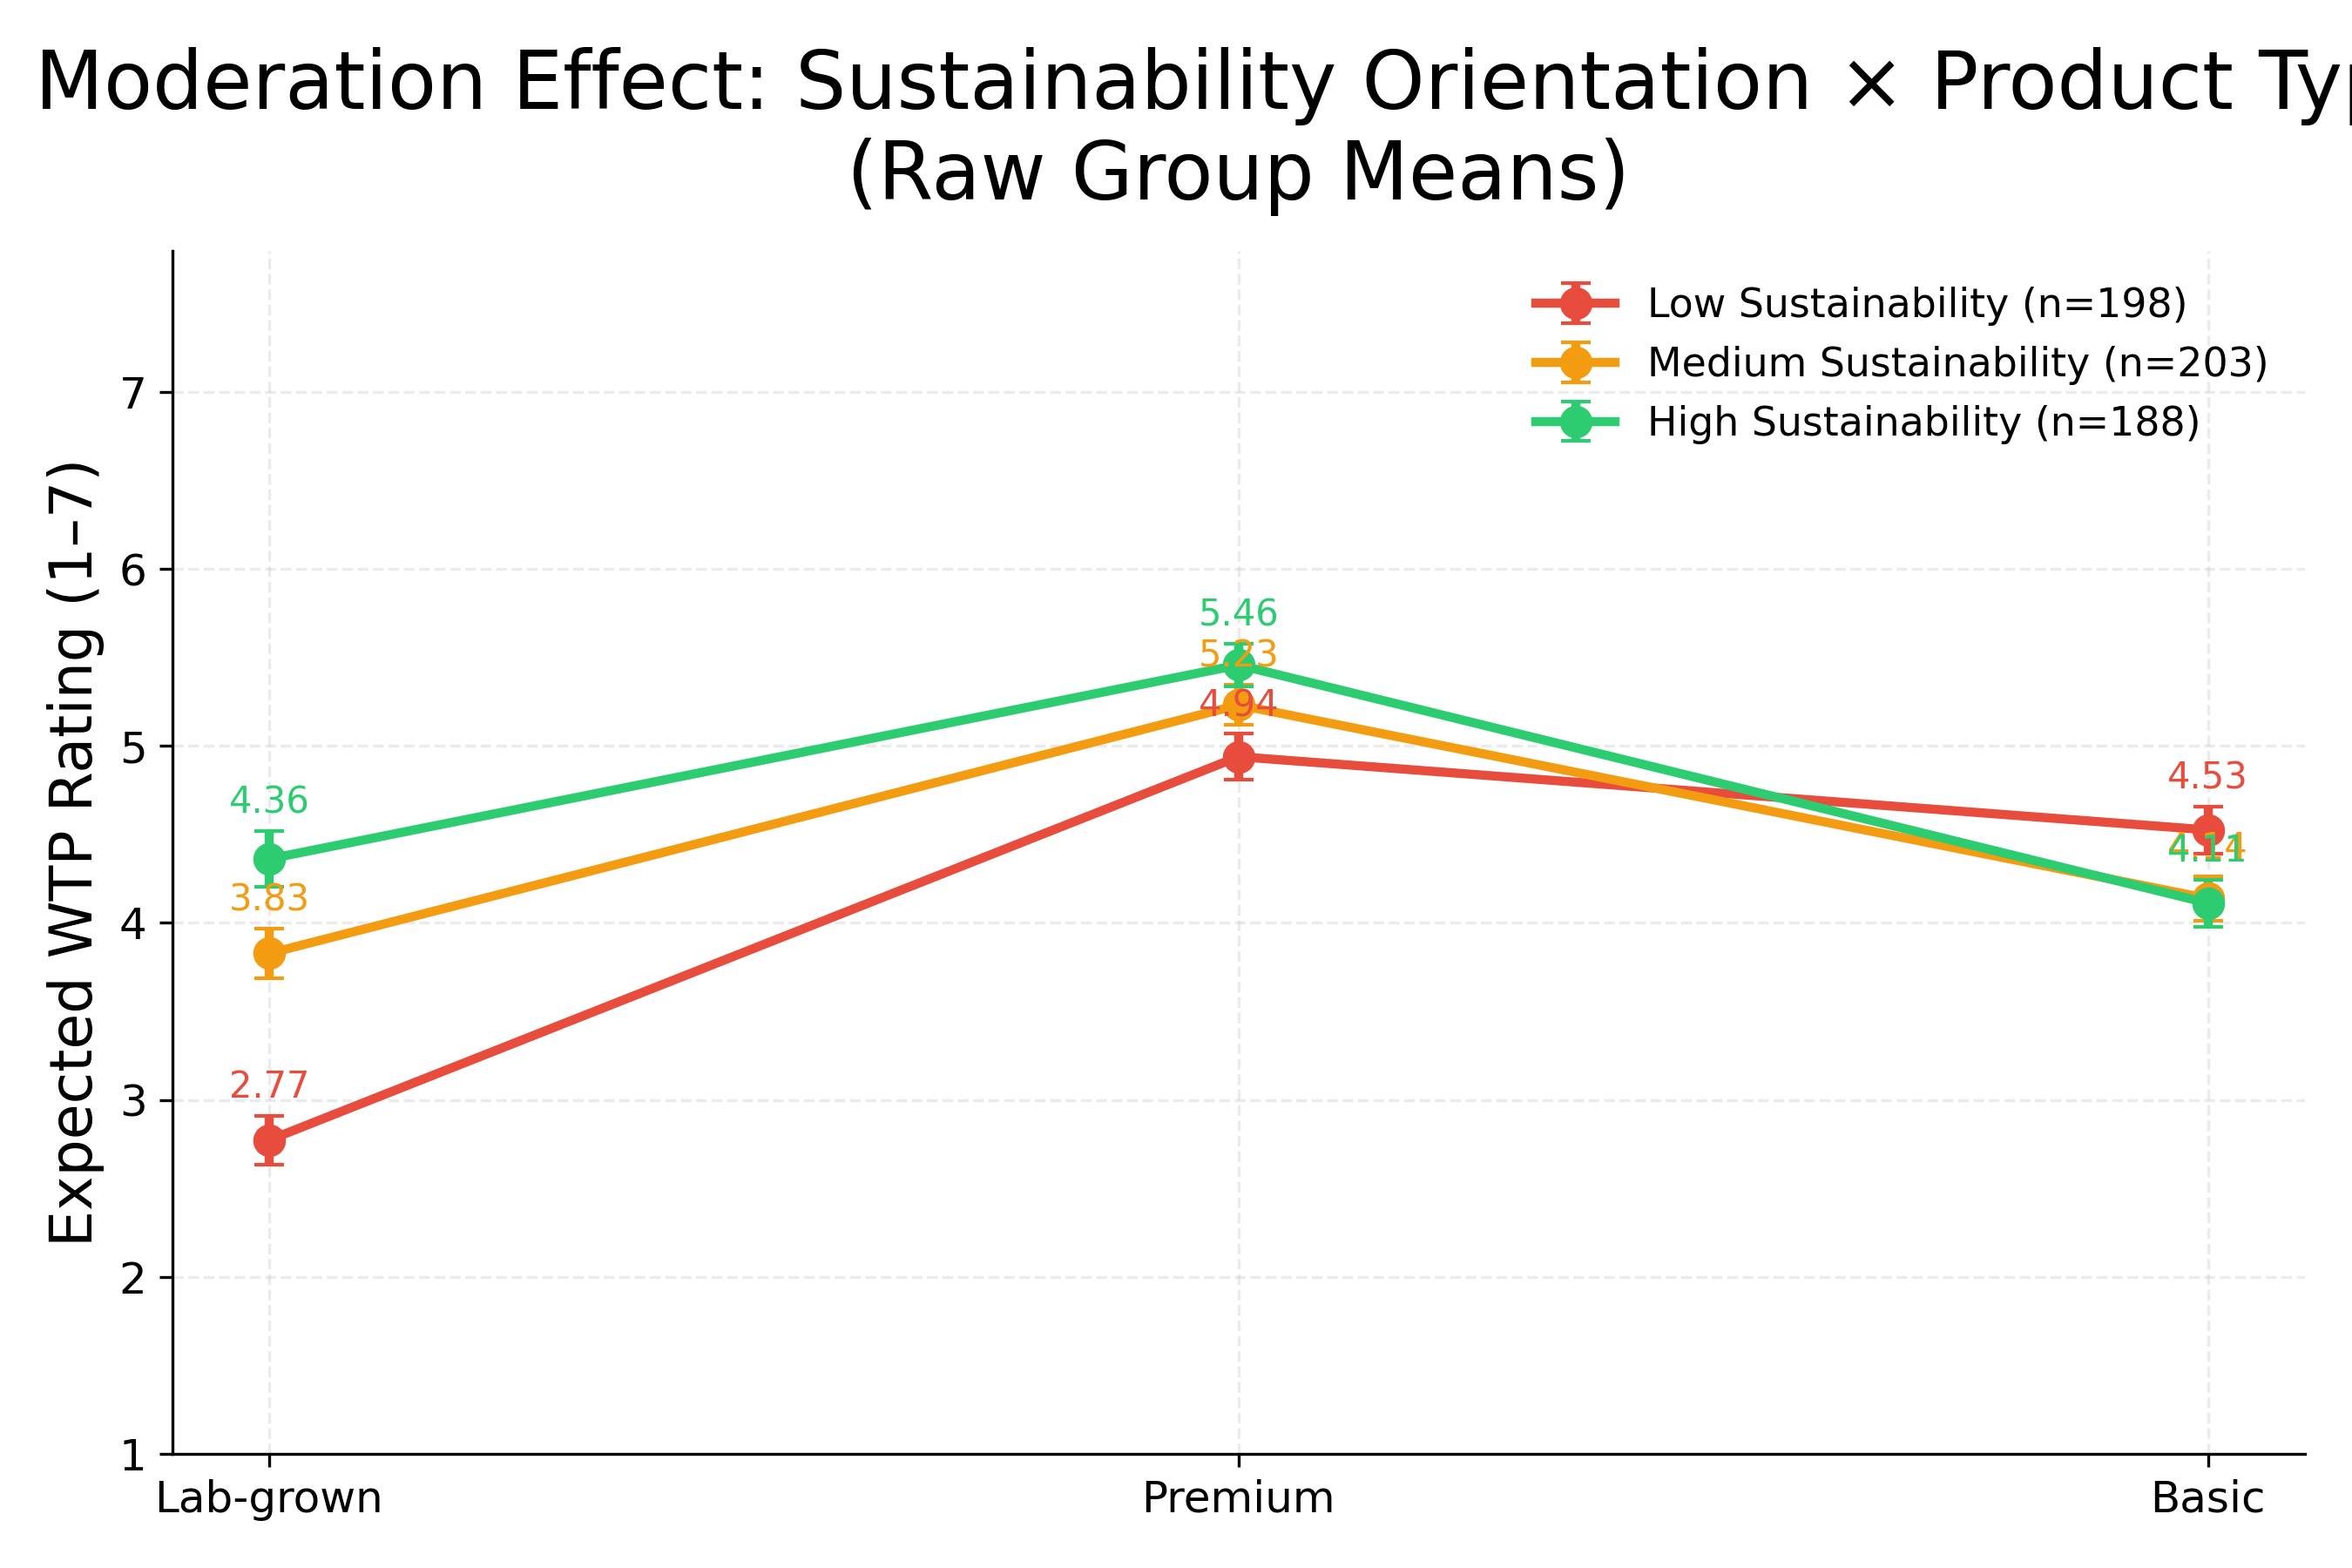
\includegraphics[width=0.95\textwidth]{figures/fig_moderation_simple_slopes.png}
\caption[Simple Slopes: Attitude × Product Type]{Simple-slopes visualization of the Attitude Score $\times$ Product Type interaction. Expected willingness-to-purchase is plotted for low, medium, and high sustainability-attitude terciles across the three product types. Lab-grown tuna shows a substantially steeper positive slope than Premium or Basic, illustrating that attitude effects are concentrated on the novel product.}
\label{fig:moderation}
\end{figure}

\paragraph{Behaviors alone do not moderate product preference.} None of the Behavior~Score~$\times$~X interactions (with Product, Nutrition, Taste, Health Label, Price, or Education) reached significance ($p>.10$ in every case). This cleanly separates the theoretical contributions of values and actions in the attitude--behavior gap literature: it is \textit{what consumers believe about sustainability}, not \textit{what they report doing}, that predicts openness to genuinely novel products like lab-grown tuna. Self-reported sustainable behavior appears to index conventional eco-conscious consumption (e.g., reusable packaging, organic produce) rather than willingness to adopt disruptive food technologies.

\paragraph{Education amplifies lab-grown acceptance.} A previously underappreciated demographic moderator emerged in this analysis. The Lab-grown~$\times$~Education interaction was significantly positive ($\beta=+0.220$, $SE=0.081$, $t=2.72$, $p=.006$), indicating that for each additional year of formal education, lab-grown WTP increases by an extra 0.22 points beyond the main effect. The Premium~$\times$~Education interaction was non-significant, again pointing to a Lab-specific moderation. Education appears to function similarly to Attitude here: it indexes the kind of cognitive engagement and informational openness that lowers resistance to novel food technology.

\paragraph{Product--attribute interactions favor strong differentiation.} Three product--by--attribute interactions reached significance: Lab~$\times$~Nutrition~High ($\beta=+0.458$, $p<.001$), Premium~$\times$~Nutrition~High ($\beta=+0.575$, $p<.001$), and Premium~$\times$~Taste~High (also $\beta=+0.575$, $p<.001$). High nutrition claims boost both lab-grown and premium tuna disproportionately, while high taste claims specifically lift premium tuna. Conversely, Lab~$\times$~Taste~Mid was significantly negative ($\beta=-0.858$, $p<.001$): mid-level (i.e., merely-acceptable) taste claims actively suppress lab-grown WTP, suggesting that for novel products, ambiguous taste signals raise more doubt than they resolve.

% ------------------------------------------------------------------------
% 5.5 Scenario Interactions: Price-Nutrition Trade-offs
% ------------------------------------------------------------------------
\subsection{Scenario Interactions: Price--Nutrition Trade-offs}\label{subsec:scenario-interactions}

The Price Level $\times$ Nutrition Level block was the strongest set of scenario-attribute interactions in Model~2. Three of four cells reached significance.

\paragraph{High nutrition justifies mid-to-high pricing.} Mid price $\times$ High nutrition produced the largest positive synergy ($\beta=+0.529$, $SE=0.082$, $p<.001$), and High price $\times$ High nutrition also showed a substantial boost ($\beta=+0.435$, $p<.001$). Substantively: when high nutritional claims accompany elevated price points, WTP increases \textit{above} what would be predicted from additive main effects---consumers treat high nutrition and non-low pricing as mutually reinforcing quality signals.

\paragraph{Mid price $\times$ Mid nutrition suppresses WTP.} In contrast, Mid price paired with Mid nutrition showed a significant negative interaction ($\beta=-0.257$, $p=.013$), indicating that ``average across the board'' positioning underperforms additive expectations. Consumers appear to reward differentiation (high on one dimension, any on the other) and penalize mediocrity on multiple dimensions simultaneously.

\paragraph{Product-specific price sensitivity was not detected.} PriceUSD $\times$ Product interactions were non-significant for both Lab ($\beta=-0.153$, $p=.138$) and Premium ($\beta=+0.042$, $p=.706$), suggesting that the per-dollar price slope does not differ meaningfully across product types once their baseline price positions are controlled for. Lab Price Gap $\times$ Product interactions were also non-significant. We interpret this as evidence that the large mean-level differences in WTP across products (Section~\ref{subsec:main-effects}) are driven primarily by product-attribute perceptions rather than differential price responsiveness.

% ------------------------------------------------------------------------
% 5.6 Pre/Post Health-Label Comparison
% ------------------------------------------------------------------------
\subsection{Pre/Post Health-and-Safety-Label Comparison}\label{subsec:healthlabel}

The April 2026 wave incorporated a key design addition relative to September 2025: a prominent health-and-safety label was displayed above the product-attribute card. Scenarios held Basic tuna at \$2.50 and Premium tuna at \$4.50 while varying lab-grown price across five levels (\$1.50--\$5.50), enabling identification of the lab-grown price slope independent of the conventional alternatives. We include a HealthLabel binary indicator to capture the wave-level intervention effect, with follow-up analyses decomposing its components.

\paragraph{Label main effect.} The HealthLabel omnibus test was significant ($F(1)=9.89$, $p=.002$), and the Yes/No contrast in Model~1 was $\beta=-0.590$ ($SE=0.189$, $p=.002$). This main effect reads primarily as a wave-level adjustment rather than a direct effect of the label itself; the label's substantive influence manifests through its interaction with price, reported below.

\paragraph{HealthLabel moderates price sensitivity.} In the unified Model~2 (Table~\ref{tab:glm_interactions}), the Health-and-Safety-Label~$\times$~Price~(USD) interaction reached significance ($\beta=+0.320$, $SE=0.153$, $t=2.09$, $p=.037$). Interpreted directionally: in the September~2025 wave (no health label), the per-dollar price slope was steeply negative; in the April~2026 wave (with health label), the slope was offset by approximately +0.32 per dollar, attenuating consumer price sensitivity. The health and safety label appears to dampen consumer responsiveness to price increments---once safety is signaled, dollar increases carry less deterrent weight. This finding has direct policy implications: voluntary or regulatory health-certification schemes may extend the price ceiling at which novel-protein products remain commercially viable. Other HealthLabel interactions (with Product, Nutrition, Taste, Attitude, Behavior, Education) did not reach significance in the unified model.

\paragraph{Label $\times$ product type: descriptive only.} Although the formal Product~$\times$~HealthLabel interactions did not reach significance in Model~2, the descriptive shift between waves (Figure~\ref{fig:healthlabel}) shows Lab-grown WTP increasing by approximately +0.67 points while Basic and Premium remained essentially flat. This pattern is consistent with the mechanism implied by the significant Label~$\times$~Price interaction: when uncertainty about novel-product safety is reduced via a credible health endorsement, consumers become less price-deterred specifically when evaluating the product where uncertainty is highest (lab-grown).

\begin{figure}[ht]
\centering

\includegraphics[width=0.95\textwidth]{figures/fig_healthlabel_interactions.png}
\caption[Health Label Interaction Effects]{Health-and-safety-label manipulation effects. \textbf{Panel A:} HealthLabel $\times$ PriceUSD interaction. Regression lines show per-dollar price slopes separately for the September 2025 wave (no label) and the April 2026 wave (with label). The presence of the health label flattens the price-sensitivity slope ($p=.007$). \textbf{Panel B:} HealthLabel $\times$ Product Type descriptive comparison. Bars show mean WTP by product with and without the label; Lab-grown shows the largest positive shift ($\Delta=+0.67$), while Basic and Premium remain largely unchanged.}
\label{fig:healthlabel}
\end{figure}

% ------------------------------------------------------------------------
% 5.7 Robustness Check: Ordered Logit Sensitivity
% ------------------------------------------------------------------------
\subsection{Robustness Check: Ordered Logit Sensitivity}\label{subsec:robustness}

Because willingness-to-purchase is measured on a seven-point Likert scale, we refit Model~1 as an Ordered Logit model \citep{agresti2010} as a sensitivity check. Direction agreement between OLS $\beta$ coefficients and Ordered Logit log-odds coefficients was 100\% for all 25 main-effect predictors with non-trivial OLS coefficients, and overall statistical significance patterns matched. Predictions from both models also fell entirely within the 1--7 bounded range for all observations in our data. We therefore report OLS estimates as our primary results while acknowledging that Ordered Logit yields substantively identical conclusions.

% ------------------------------------------------------------------------
% 5.8 Summary of Findings
% ------------------------------------------------------------------------
\subsection{Summary of Findings}\label{subsec:summary}

% NOTE: [H] placement requires \usepackage{float} in the main preamble.
% Without it, LaTeX will float this table to the very end of the document.
\begin{table}[H]
\caption{Summary of Key Findings}
\label{tab:results_summary}
\centering
\small
\begin{tabular}{p{3.4cm}p{10cm}}
\toprule
Domain & Key Findings \\
\midrule
\textbf{Product preference hierarchy} & Premium $>$ Basic $>$ Lab-grown on average (all pairwise $p<.05$). Lab-grown rated significantly \textit{below} Basic, not above. \\ \midrule
\textbf{Dominant scenario driver} & Nutrition Level ($F(2)=146.4$, $p<.001$) outperformed Price Level ($F=0.30$, ns) and Taste Level ($F=6.17$). High and Mid nutrition claims generated the largest attribute-level WTP lifts; Mid actually outperformed High. \\ \midrule
\textbf{Continuous price sensitivity} & PriceUSD $\beta=-0.32$ per dollar ($p<.001$). Health-and-Safety Label $\times$ PriceUSD $\beta=+0.32$ ($p=.037$): the label dampens per-dollar price sensitivity. \\ \midrule
\textbf{Core moderation finding} & Lab-grown $\times$ Attitude Score: $\beta=+0.60$ ($p<.001$). Attitudes specifically amplify lab-grown acceptance; self-reported behaviors do not moderate any product preference. \\ \midrule
\textbf{Education moderation (new)} & Lab-grown $\times$ Education: $\beta=+0.22$ ($p=.006$). More-educated consumers show disproportionately stronger lab-grown WTP. Education-Premium interaction non-significant. \\ \midrule
\textbf{Product--attribute synergy} & Lab/Premium $\times$ Nutrition~High both significant; Premium $\times$ Taste~High significant; Lab $\times$ Taste~Mid significantly \textit{suppresses} WTP --- ambiguous claims hurt novel products. \\ \midrule
\textbf{Health-and-safety label} & Significant negative main effect ($\beta=-0.590$, $p=.002$, partially absorbing wave indicator). Significantly moderates per-dollar price sensitivity ($\beta=+0.320$, $p=.037$). \\ \midrule
\textbf{Demographics} & Otherwise null. All demographics except education failed to predict WTP after controlling for sustainability scores; education is significant both as main effect and as moderator of lab-grown preference. \\ \midrule
\textbf{Robustness} & Ordered-logit refit yielded 100\% direction agreement with OLS. No out-of-bounds predictions observed. \\
\bottomrule
\end{tabular}
\end{table}
